
\begin{frame}
	
	\frametitle{Empirical evaluation}
	\framesubtitle{Evaluation Metrics}
	
	\begin{itemize}	
		\item<only@1>  $\mathit{Precision} =$ $ \mathit{\frac{\#\ of\ correct\ predictions}{\#\ of\ total\ predictions}}$. The fraction of the predictions that are correct.     
		\item<only@1> $\mathit{Spread}\ $=$\ end(I) -start(I)$. The width of the prediction interval $I$, which represents the number of events between the start and the end of $I$.
	
		\item<only@1> $\mathit{PS-}$score = $\alpha * precision + (1 - \alpha ) * ( 1- \frac{spread}{max\  spread})$. In analogy with the $F-score$ we introduce this new score to assess the performance of the system in terms of both the $\mathit{precision}$ and the $\mathit{spread}$ combined.
		\item<only@1> $\mathit{Distance}\ $=$\ start(I) - now$. The distance between the start of the prediction interval $I$ and the time of prediction is produced (now). 
		\item<only@2>  $\mathit{Cumulative\ communication}$. The number of messages, which are required to perform the distributed online learning modes to synchronize the prediction models.	
		\item<only@2> $Throughput$. The number of events processed per unit time (second).
	\end{itemize} 
	
\end{frame}


\begin{frame}
	
	\frametitle{Empirical evaluation}
	\framesubtitle{Synchronization Schemes}
	
	Our proposed system can operate in three different modes of synchronization schemes: 
	\begin{itemize}	
		\item continuous full synchronization for each incoming event (hypothetical).
		\item static scheme based on synchronizing the prediction models periodically every $b$ of input events in each stream.
		\item dynamic synchronization protocol based on making the predictors communicate their local prediction models periodically but only under condition that the divergence of the local models from a reference model exceeds a variance threshold $\Delta$ (recommended).  	   
		
	\end{itemize} 
	
\end{frame}


\subsection{Real-word Event Streams\\}

\begin{frame}
	
	\frametitle{Empirical evaluation }
	\framesubtitle{Over Real-word Event Streams}
\begin{itemize}
	
	\item<only@1> Event streams describe critical points (i.e., synopses) of moving vessels trajectories, which are derived from raw AIS messages as described in \cite{synopses1}.
	\item<only@1> $4,684,444$ critical points  in Brest, France: October 2015 to March 2016 ($\approx5000$ vessels). 
	\item<only@1>  $\mathcal{P}_1=Sailing$ with $m=2$ over $\Sigma_1=$$\{$\textit{VerySlow, Slow, Moving,  Sailing, Stopping}$\}$.  
	\item<only@2> $\mathcal{P}_2=$\textit{changeInHeading; gapStart; gapEnd; changeInHeading} with $m=1$ over $\Sigma_2=$ 
	$\{$\textit{stopStart, stopEnd, changeInSpeedStart, changeInSpeedEnd,  slowMotionStart, slowMotionEnd, gapStart, gapEnd, changeInHeading}$\}$.
	\item<only@2> All experiments are performed with setting the batch size of 100  ($b=100$), the variance threshold of 2 ($\Delta=2$), $80\%$ as PMC prediction threshold ($\theta_{p}=80\%$), and 200 for the maximum spread ($\theta_{s}=200$)
\end{itemize}
	
\end{frame}


\begin{frame}
	
	\frametitle{Results on Real-word Event Streams }
	\framesubtitle{Precision scores with respect to the number of input events over time for $\mathcal{P}_1$.}
	
	\begin{figure}[H]
		\centering
		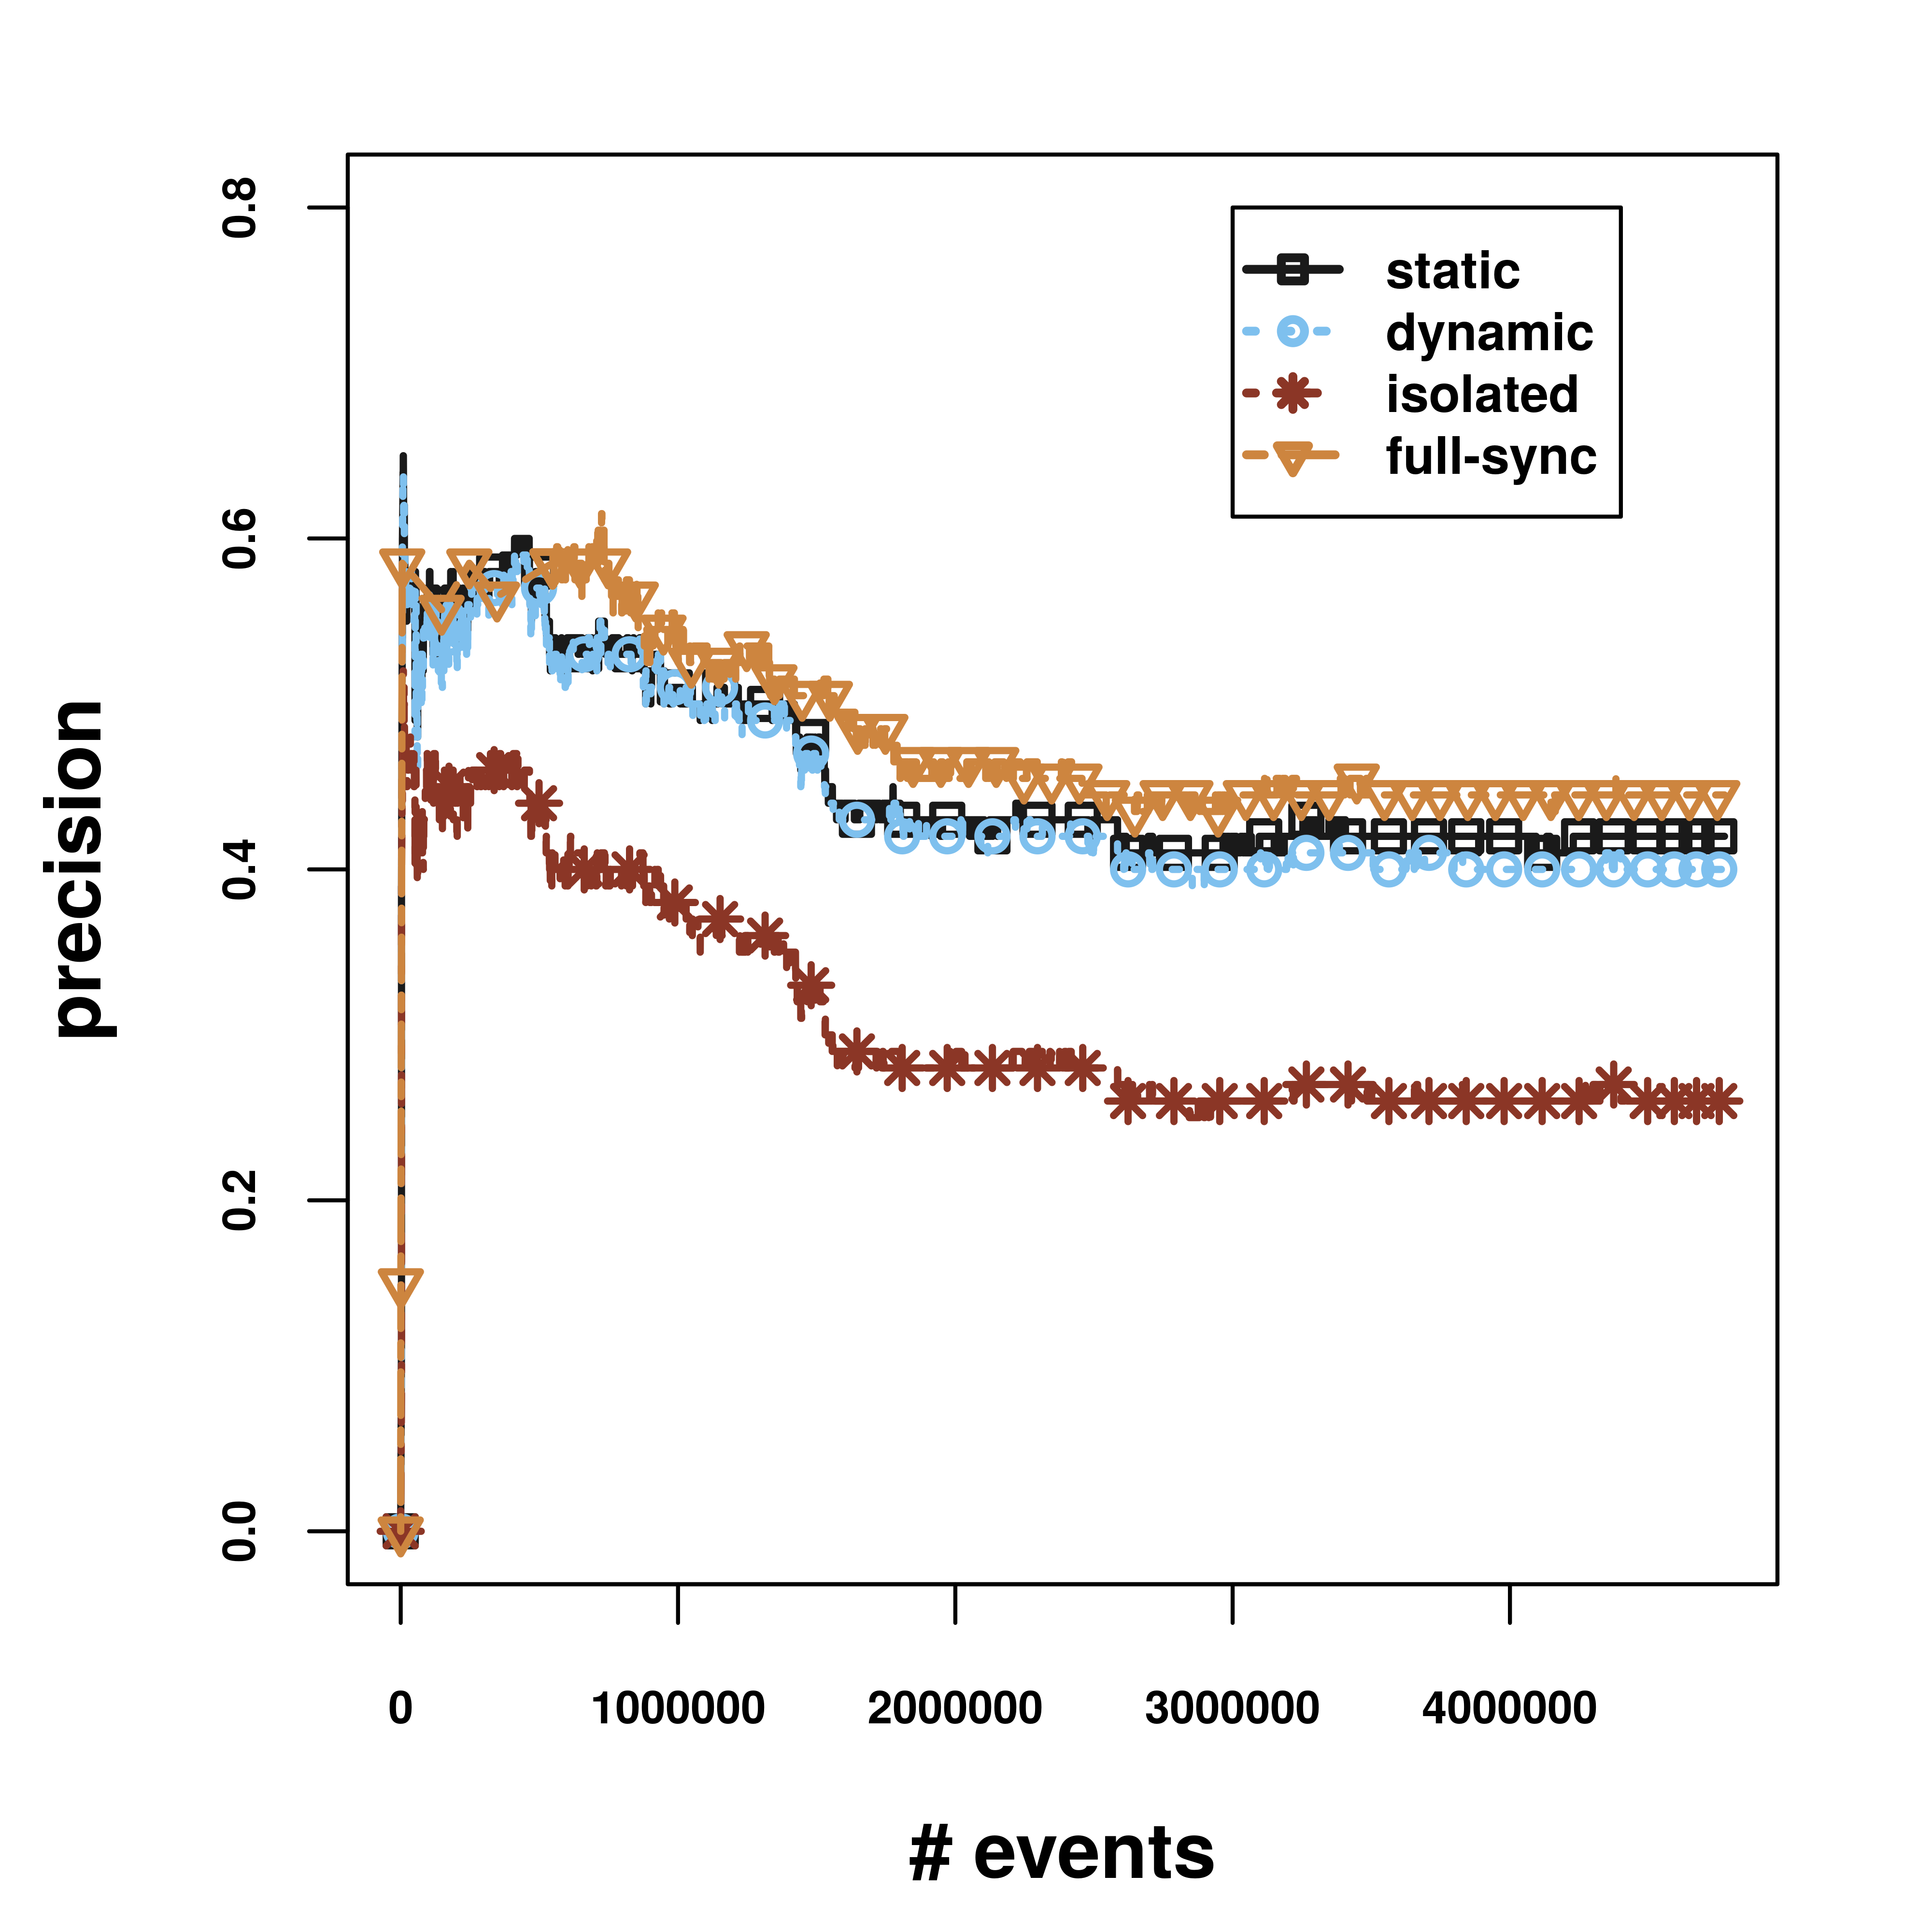
\includegraphics[width=.7\textwidth,height=.65\textheight]{../chapters/figures/synopses/new/precision_p1.png}\linebreak\\
	Methods of distributed learning outperform the isolated method.
		
	\end{figure}
	
\end{frame}



\begin{frame}
	
	\frametitle{Results on Real-word Event Streams }
	\framesubtitle{Average spread for $\mathcal{P}_1$.}
	
	\begin{center}
		
		\begin{figure}[]
			\centering
			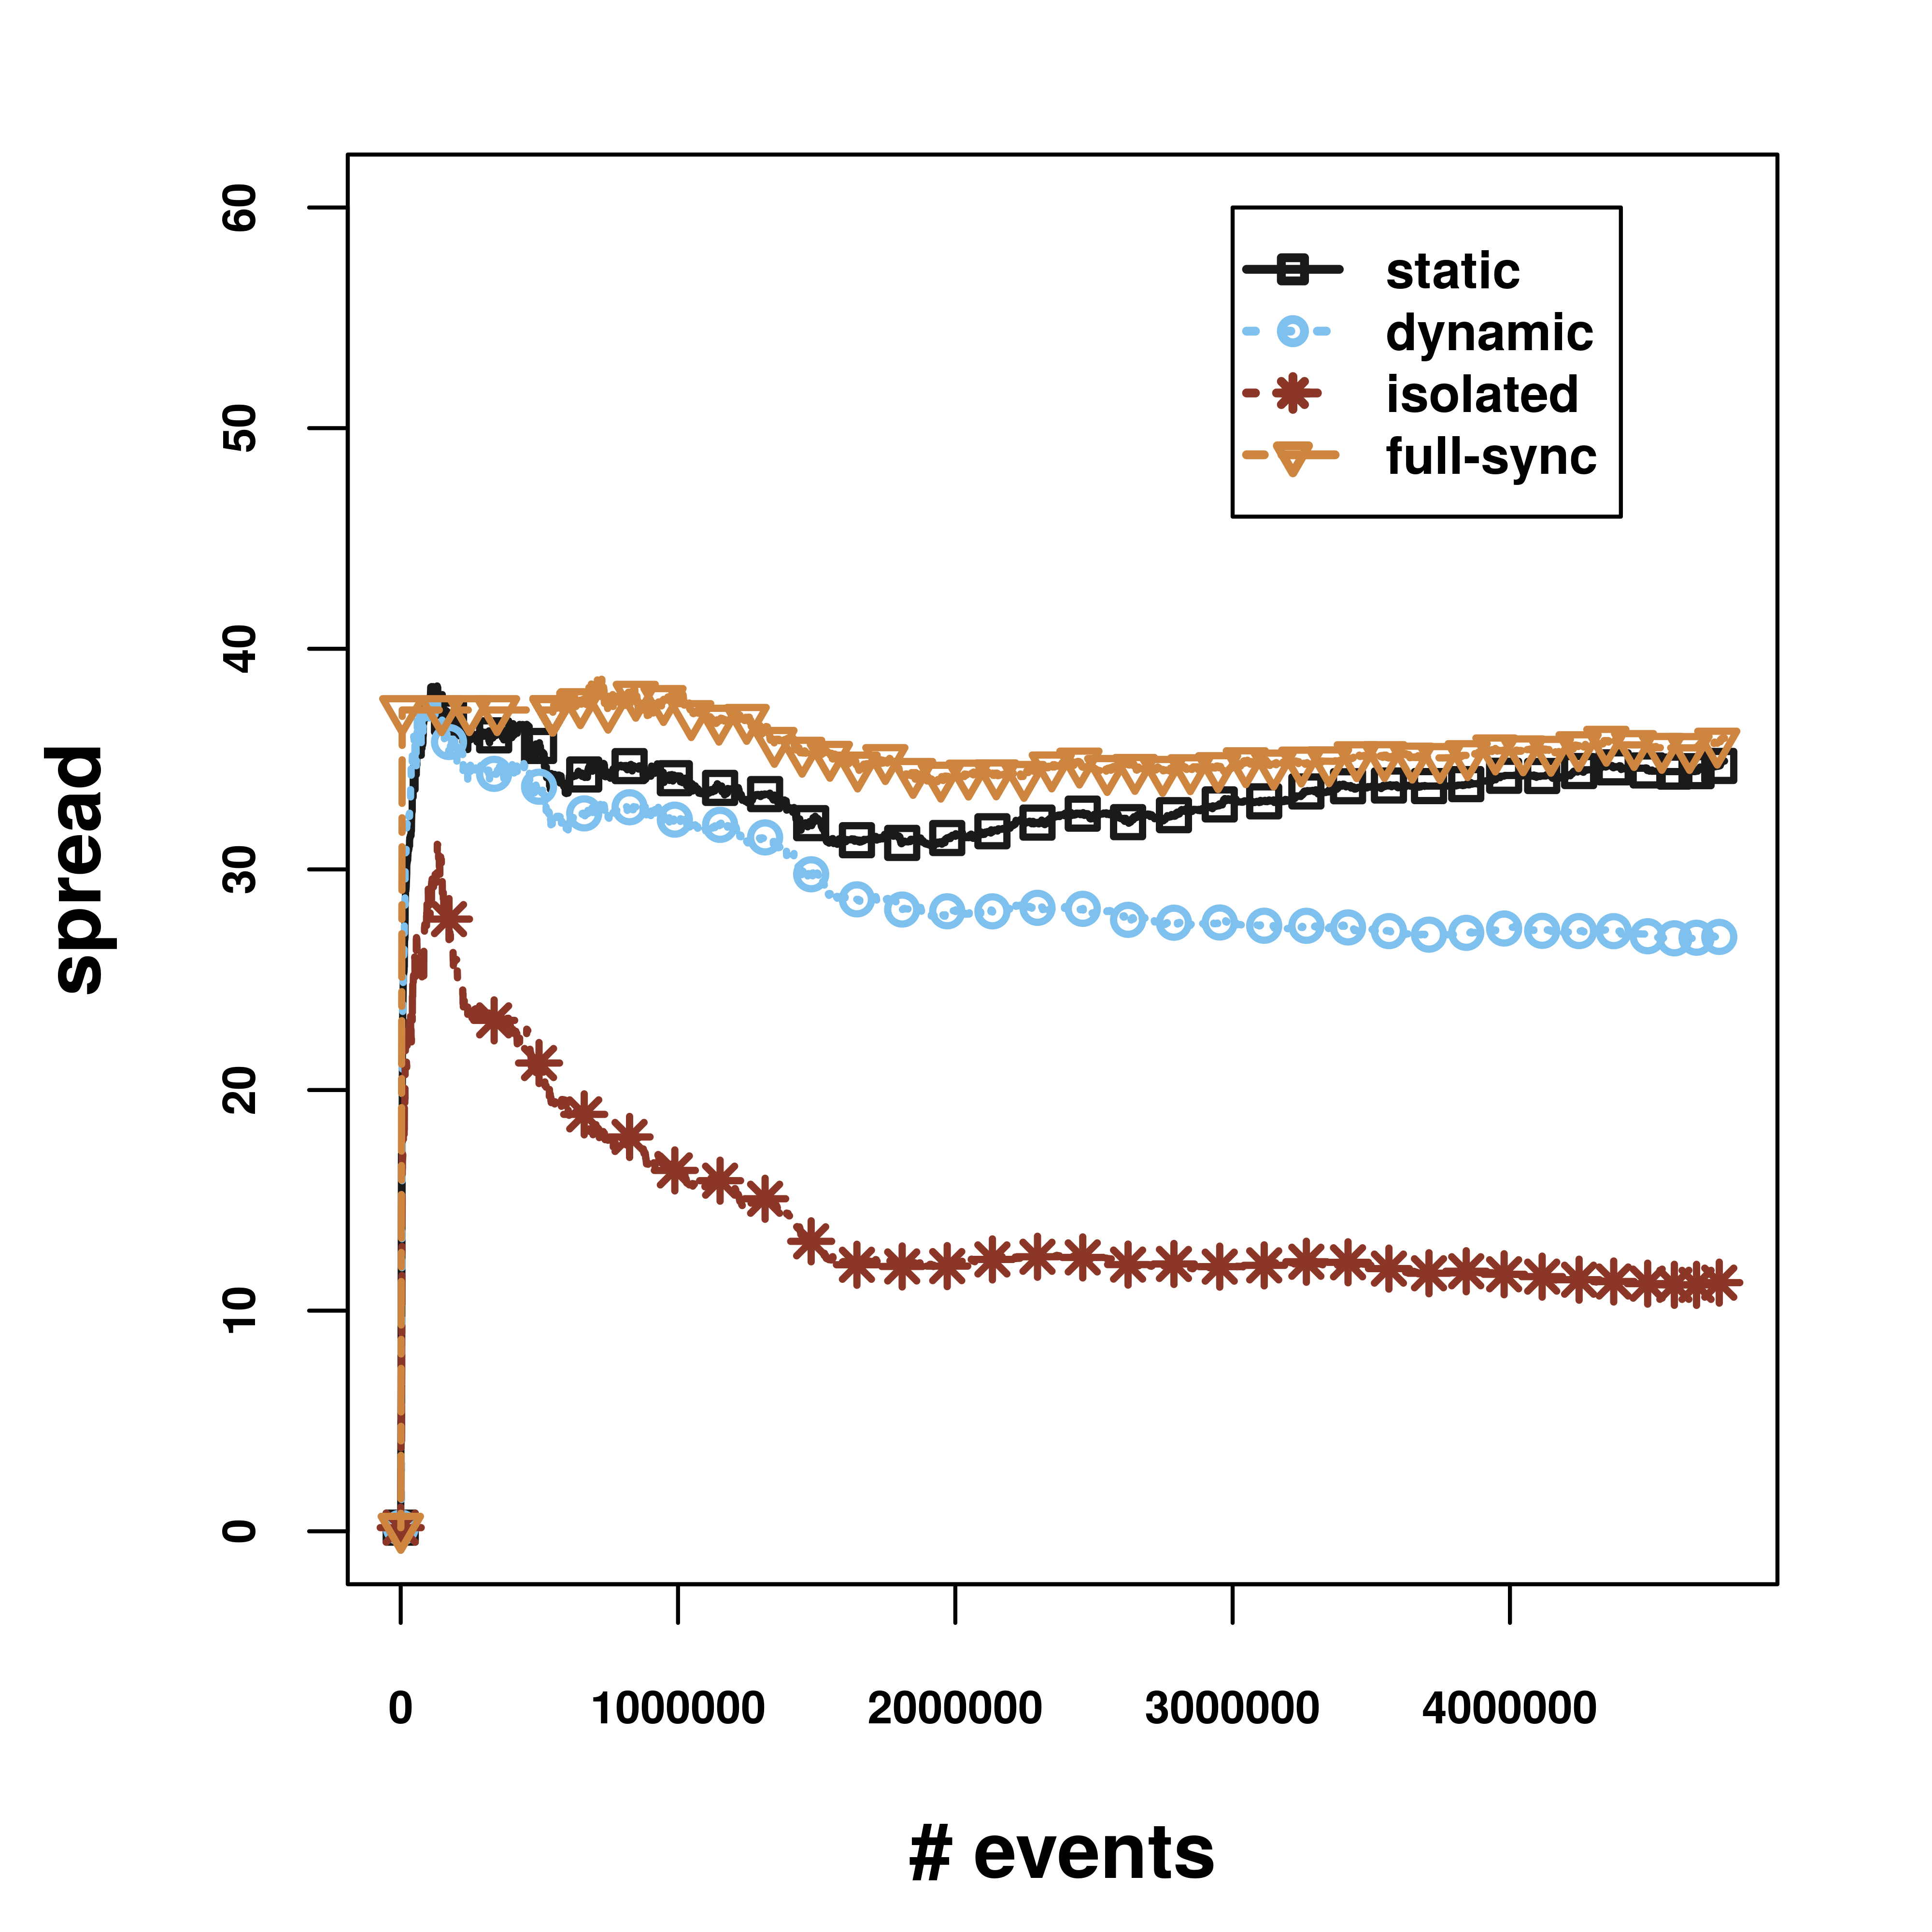
\includegraphics[width=.7\textwidth,height=.65\textheight]{../chapters/figures/synopses/new/spread_p1.png}
			
		\end{figure}
	\end{center}
	
\end{frame}


\begin{frame}
	
	\frametitle{Results on Real-word Event Streams }
	\framesubtitle{$PS$-score for $\mathcal{P}_1$ with $\alpha = .5$.}
	
\begin{center}
	\centering
	\begin{figure}[]
		
		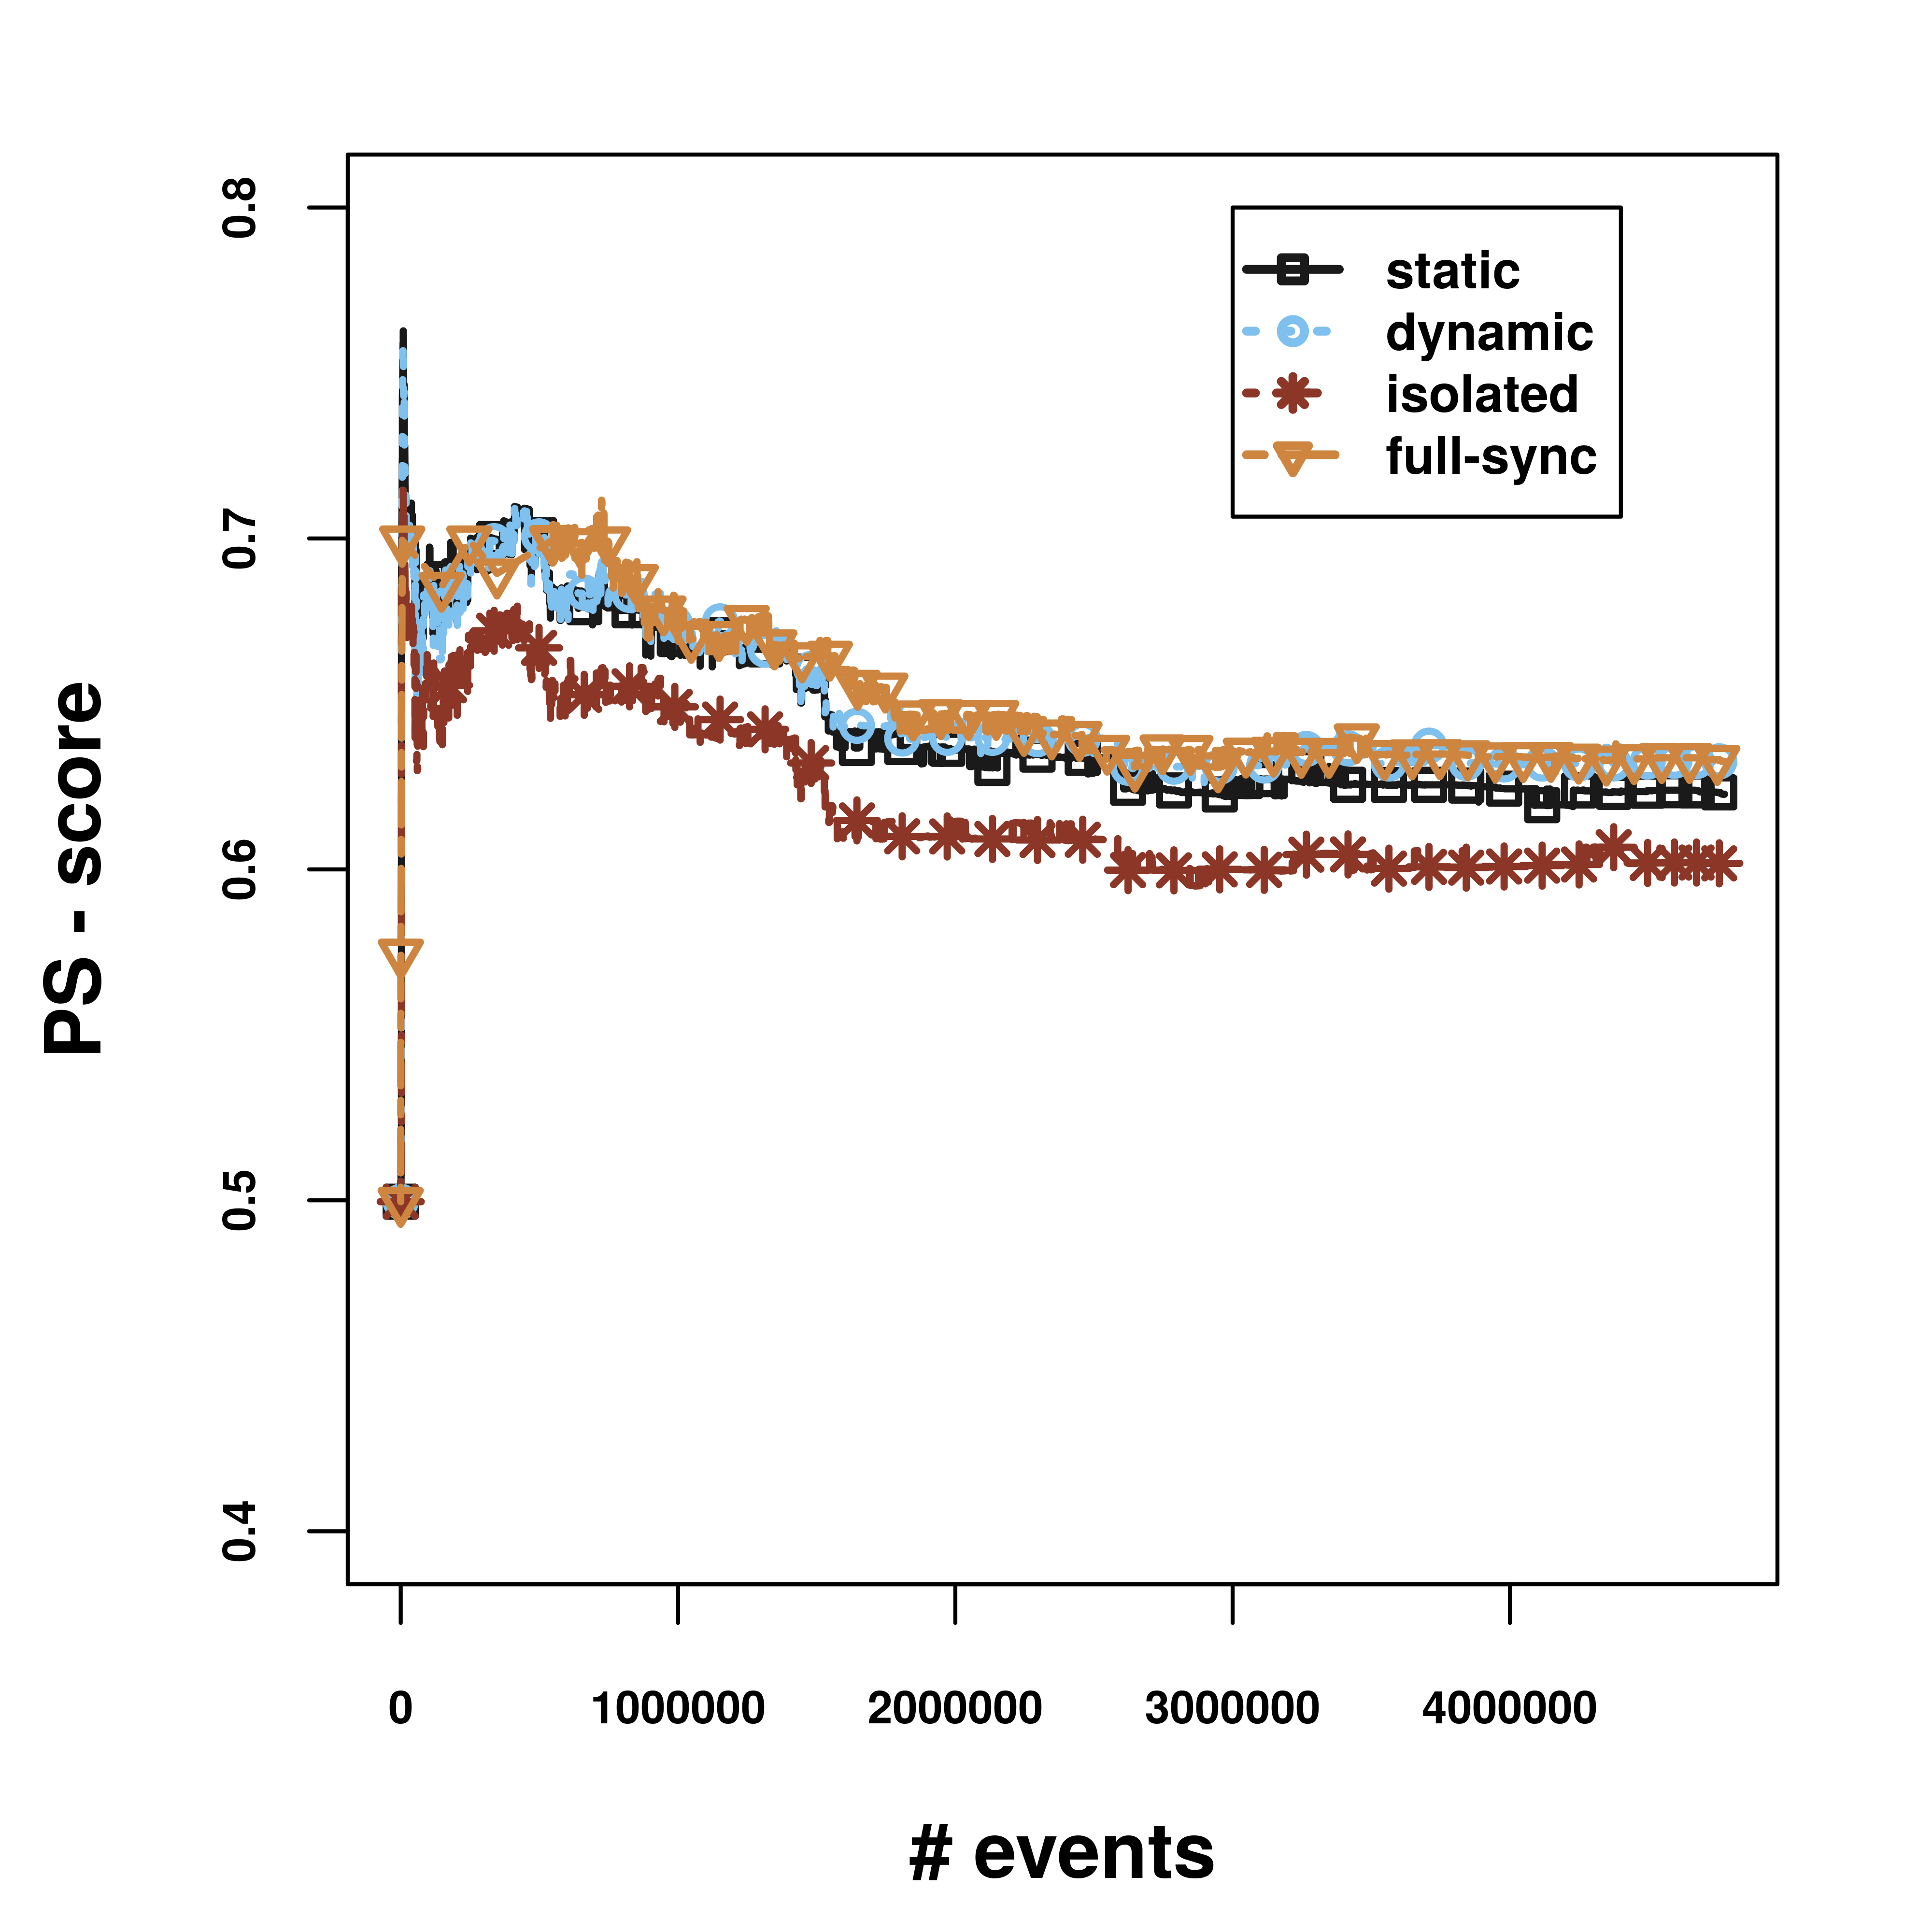
\includegraphics[width=.7\textwidth,height=.65\textheight]{../chapters/figures/synopses/new/ps_score_p1.png}
		
	\end{figure}
\end{center}
\end{frame}

\begin{frame}
	
	\frametitle{Results on Real-word Event Streams }
	\framesubtitle{Distance for $\mathcal{P}_1$.}
	
	\begin{center}
		\centering
		\begin{figure}[]
			
			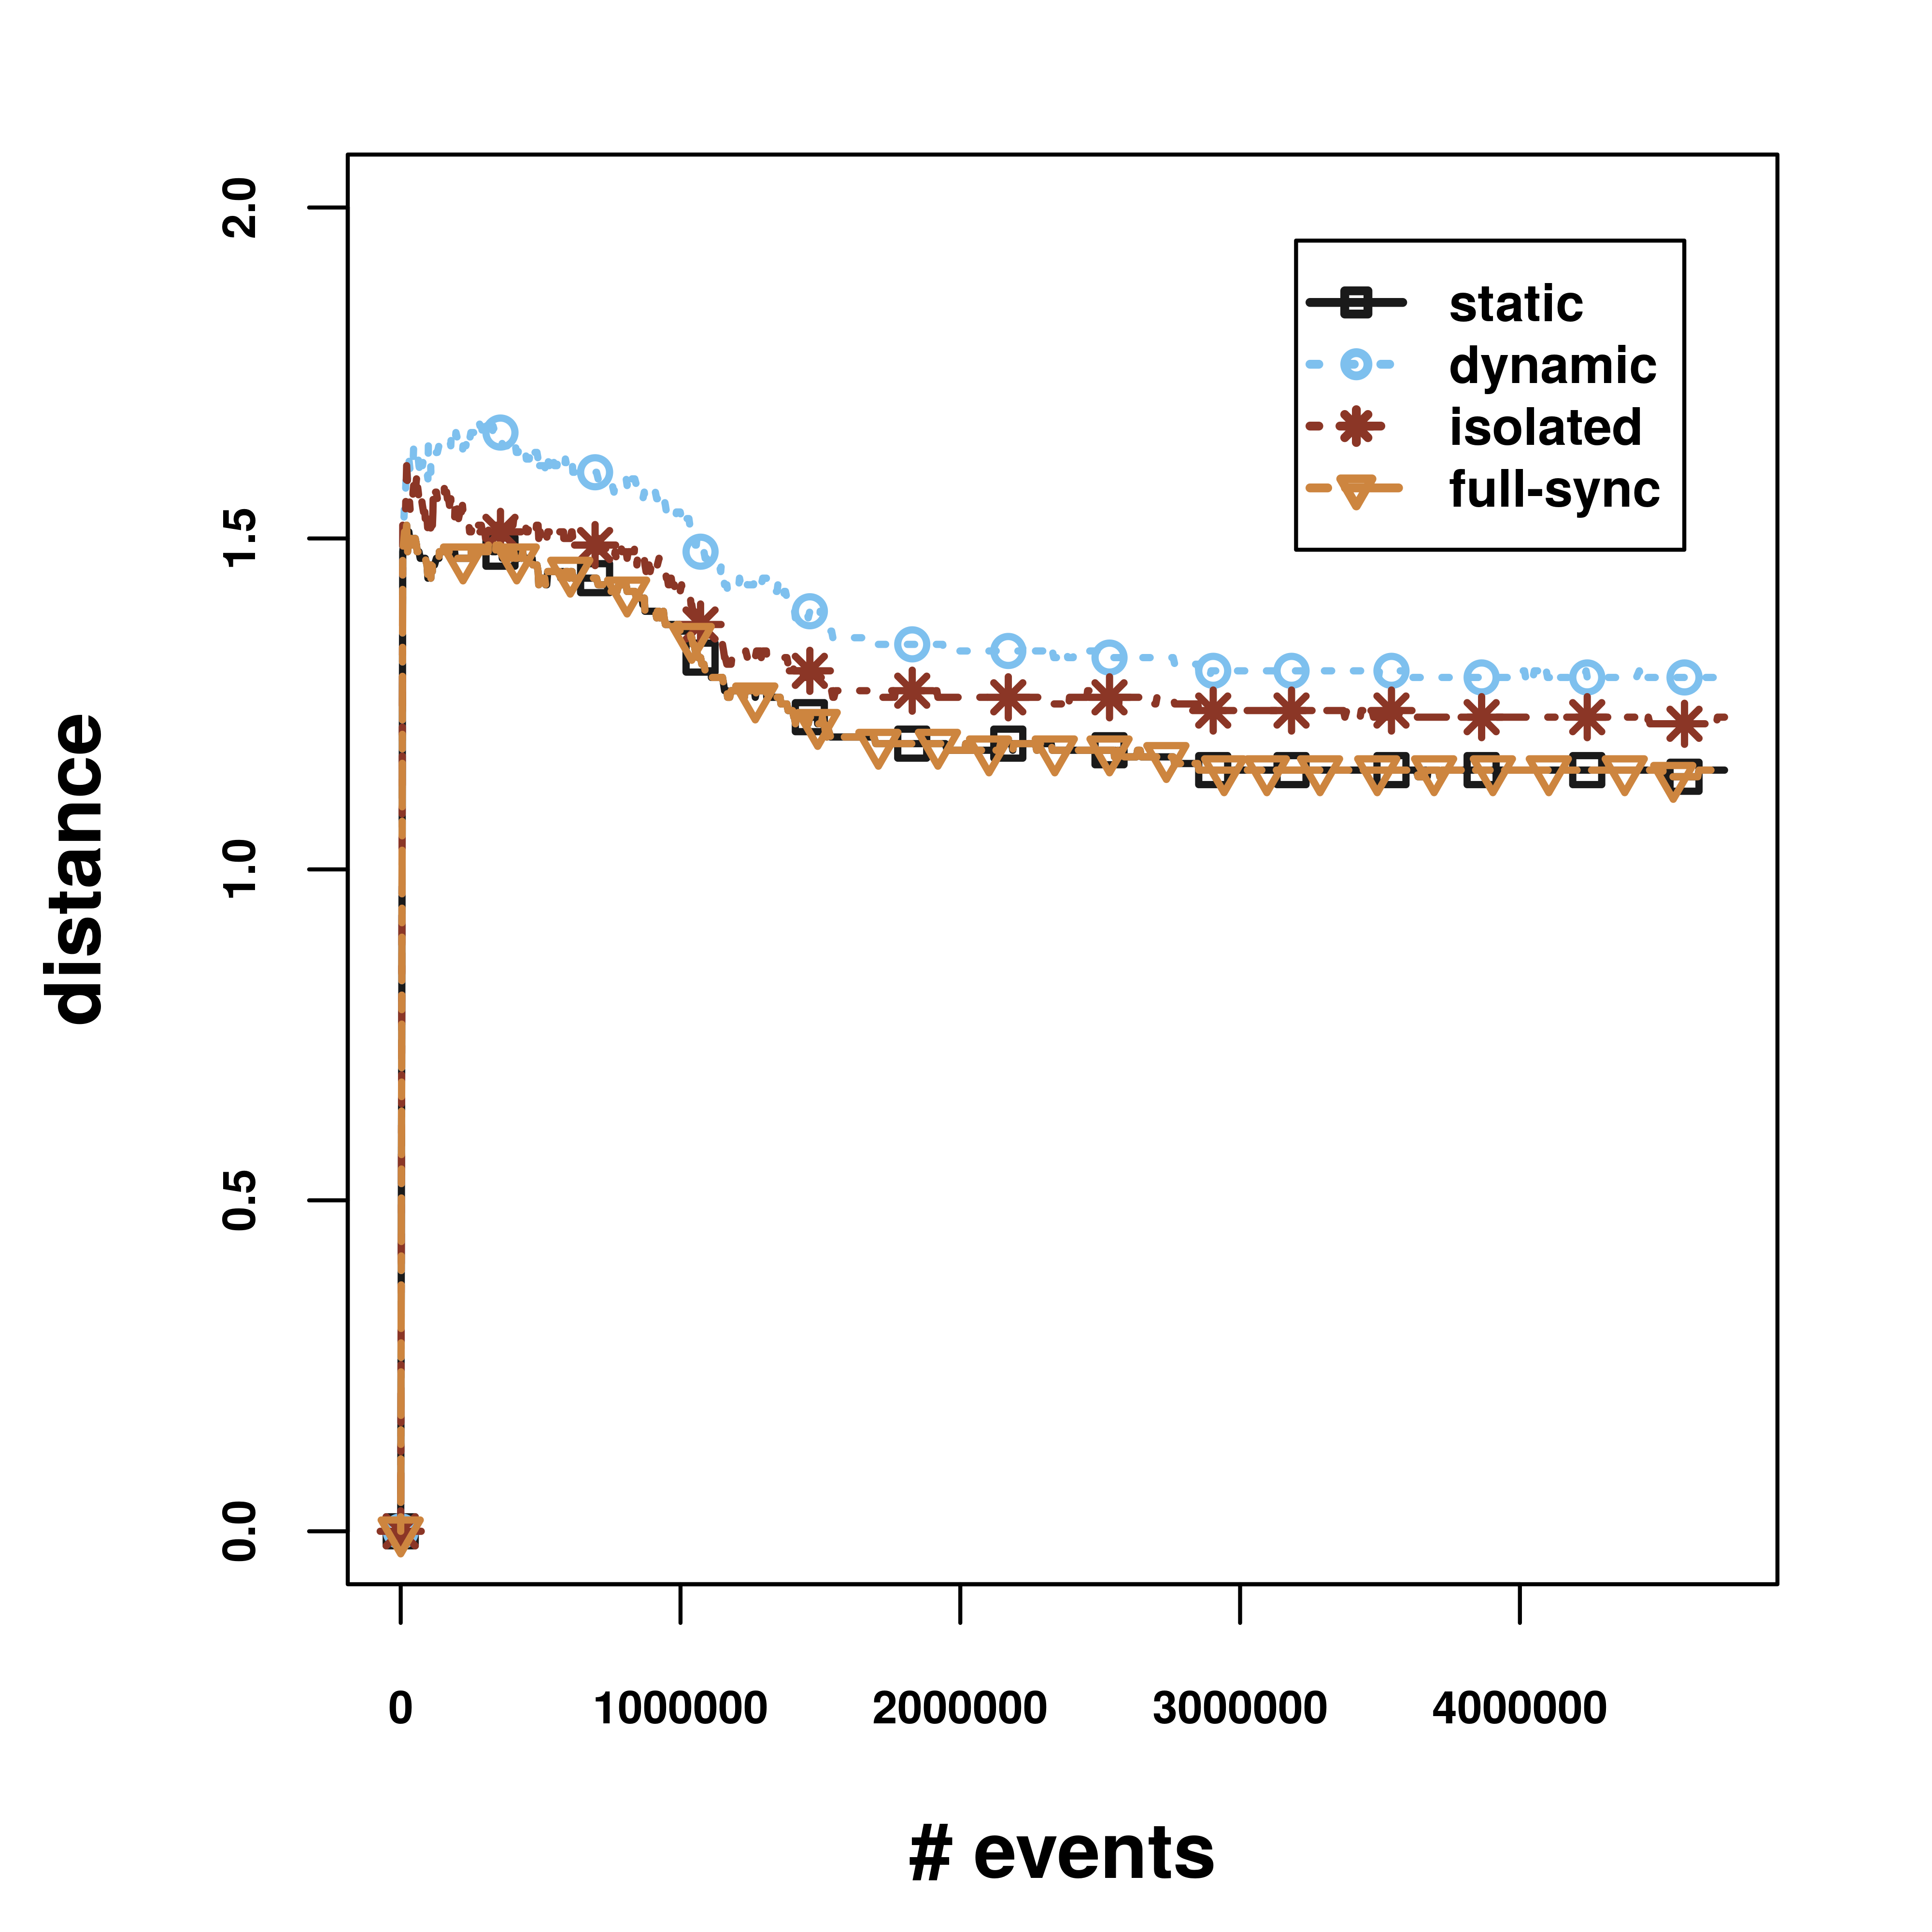
\includegraphics[width=.9\textwidth,height=.8\textheight]{../chapters/figures/synopses/new/distance_p1.png}
			
		\end{figure}
	\end{center}
	
\end{frame}

\begin{frame}
	
	\frametitle{Results on Real-word Event Streams }
	\framesubtitle{Cumulative communication with respect to the number of input events over time for $\mathcal{P}_1$.}
	
	\begin{center}
		
		\begin{figure}[]
			\centering
			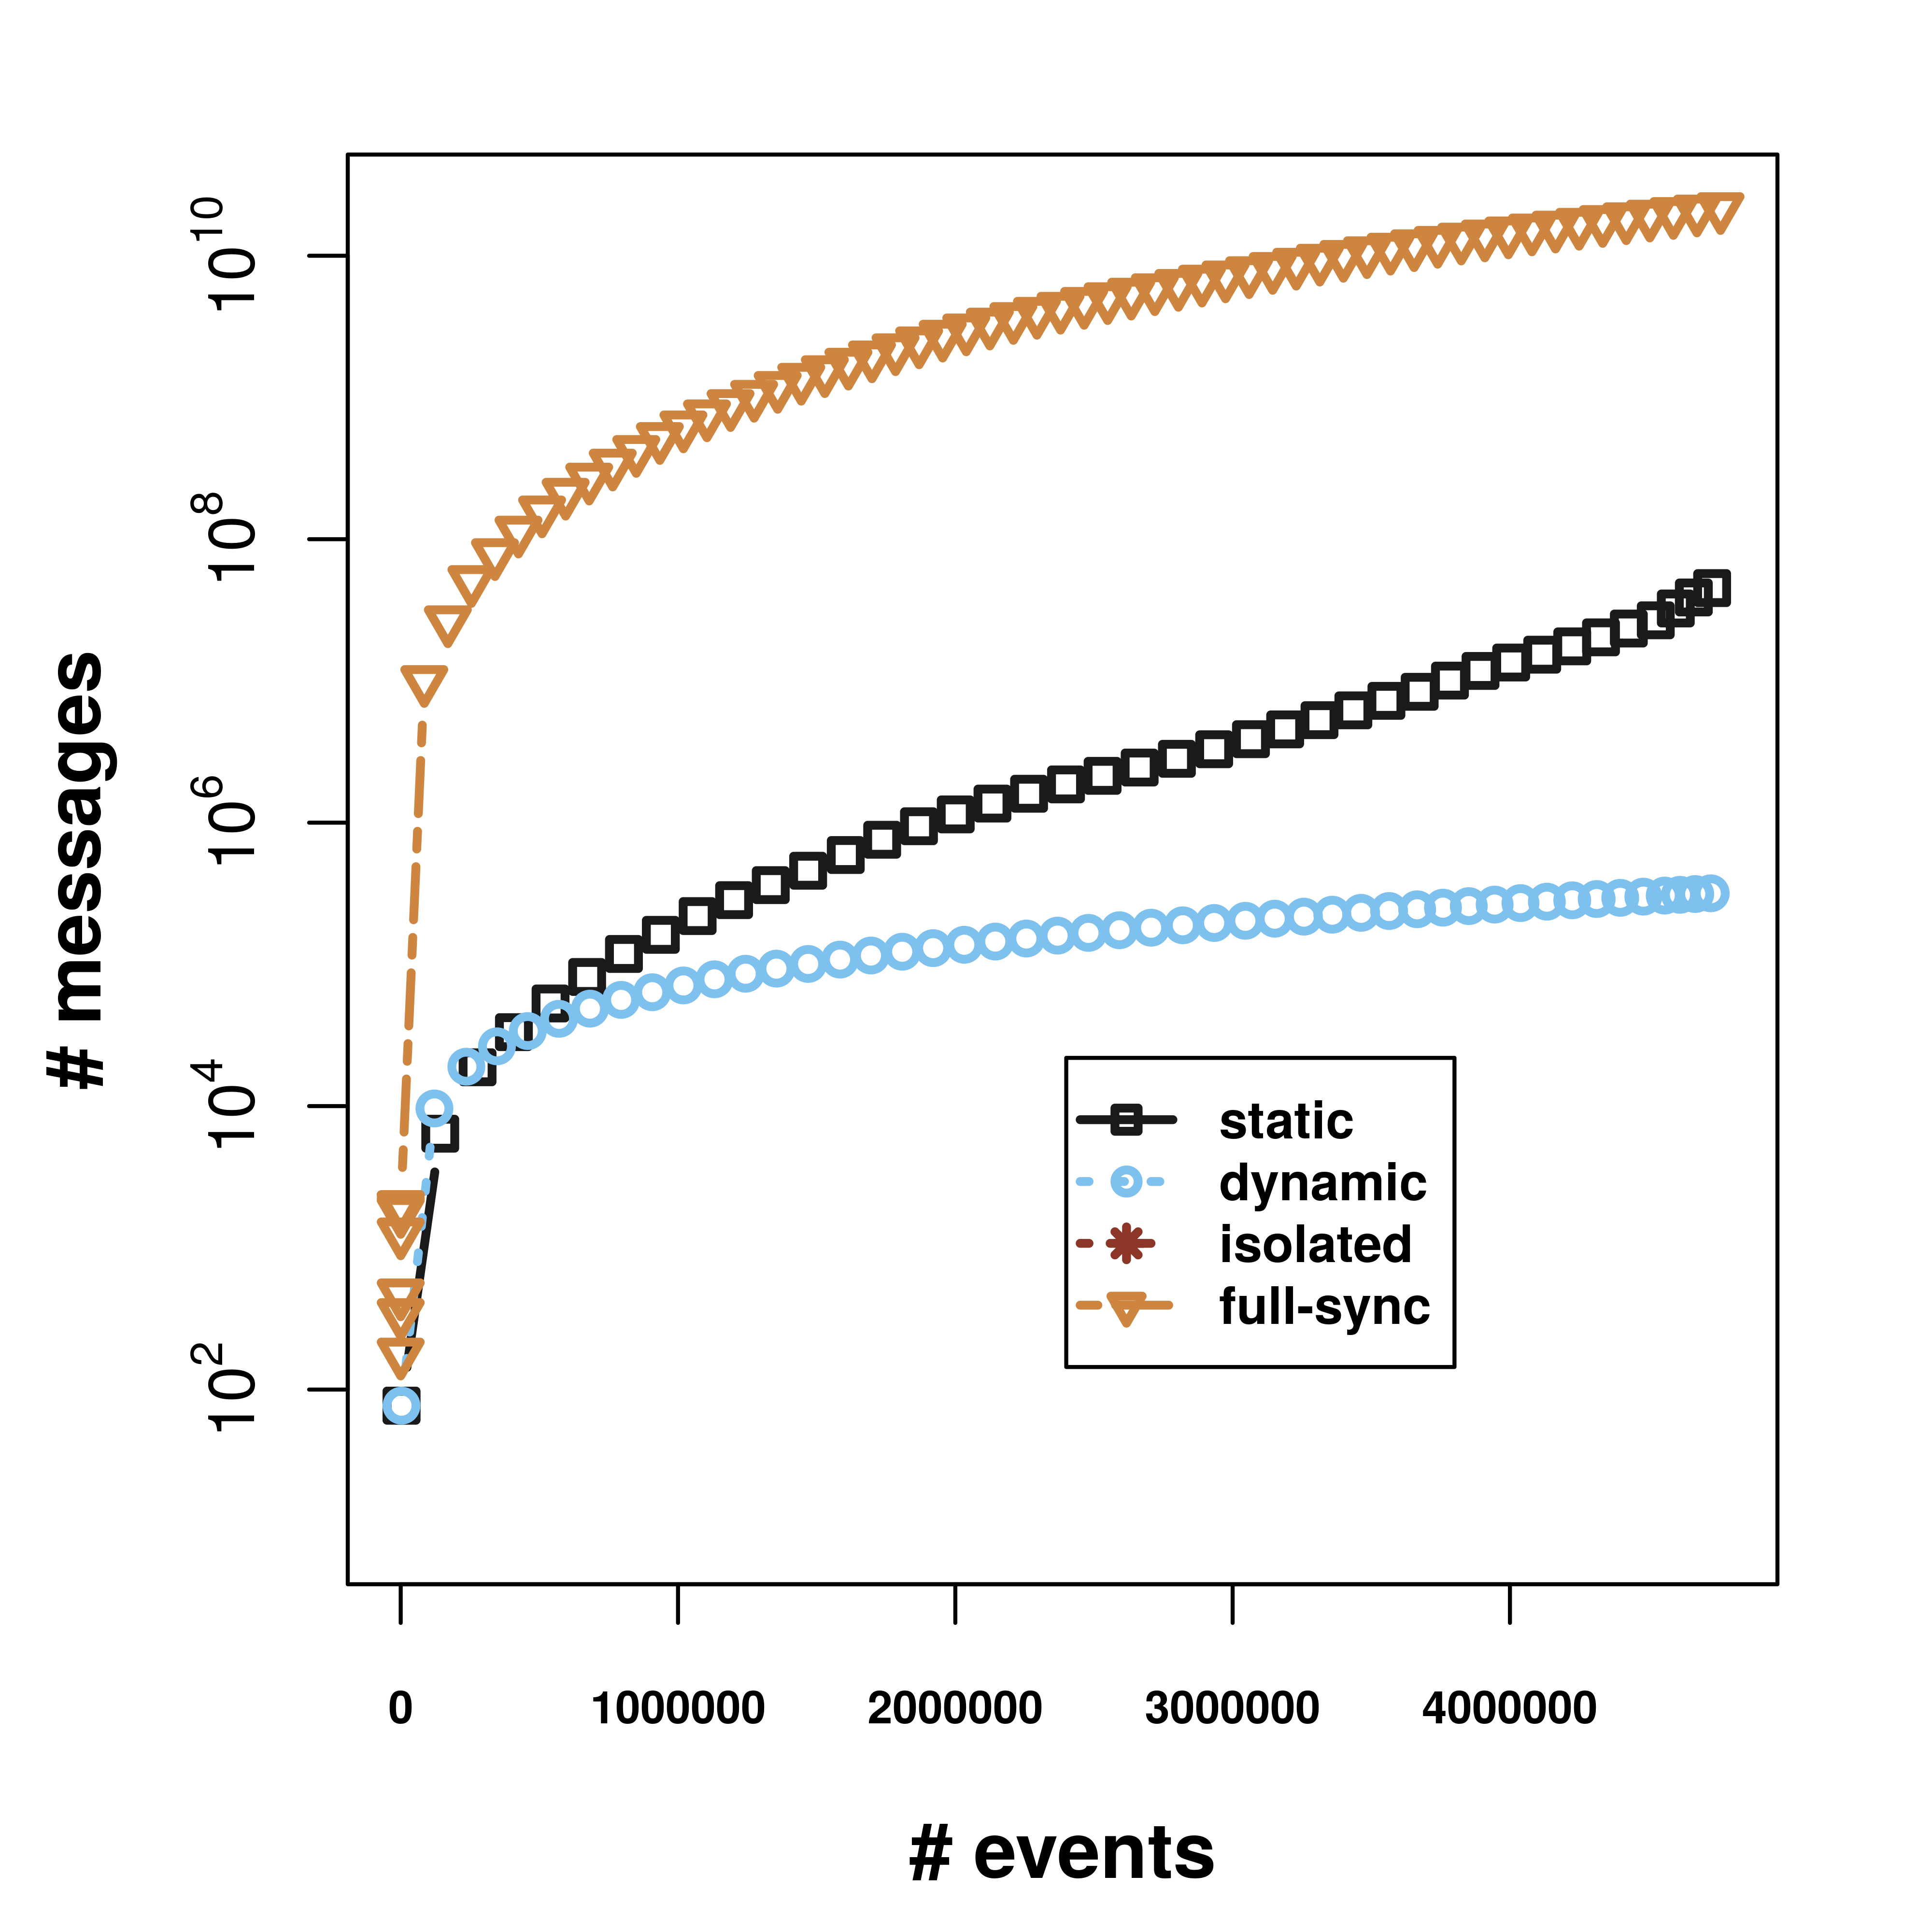
\includegraphics[width=.9\textwidth,height=.8\textheight]{../chapters/figures/synopses/new/messages_p1.png}
			
		\end{figure}
	\end{center}
	
\end{frame}


\begin{frame}
	
	\frametitle{Results on Real-word Event Streams }
	\framesubtitle{Precision scores of $\mathcal{P}_2$  for vessels of \textit{pleasure craft} type.}
	
\begin{figure}[]
	\centering
	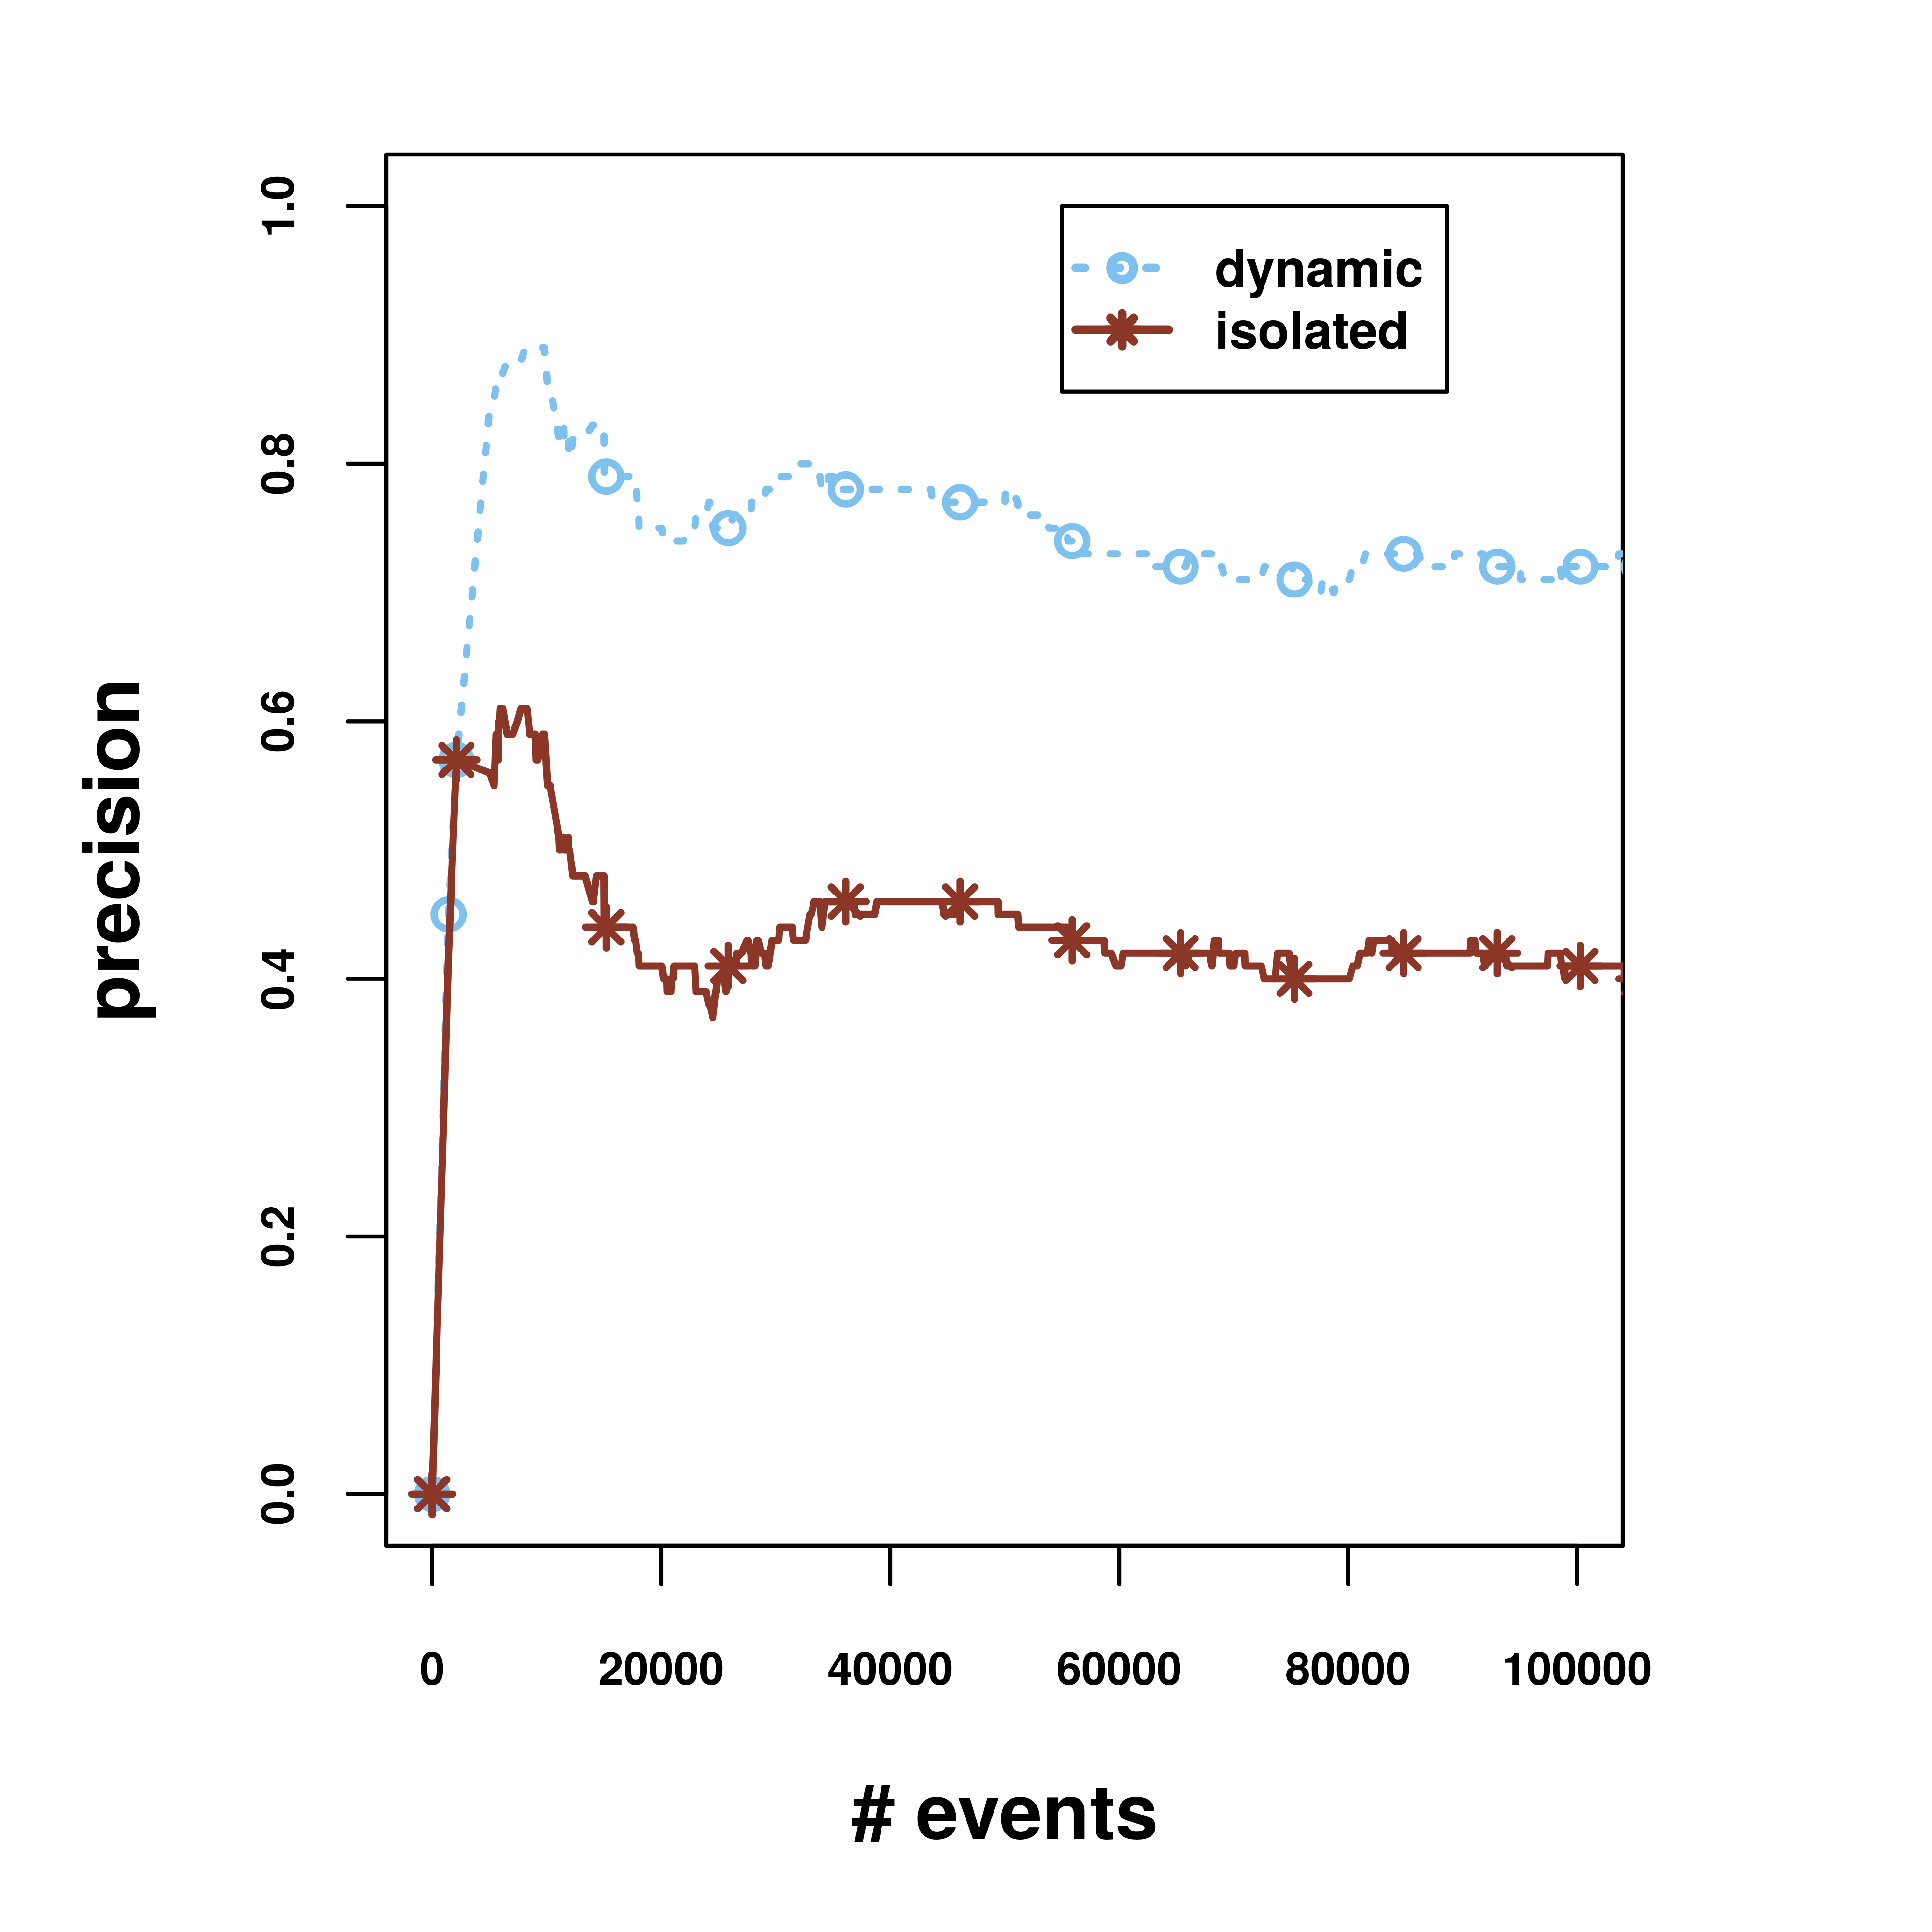
\includegraphics[width=.9\textwidth,height=.8\textheight]{../chapters/figures/synopses/new/precision_p2.png}
	
\end{figure}
	
\end{frame}



\subsection{Synthetic Event Streams}
\begin{frame}
	
	\frametitle{Empirical evaluation }
	\framesubtitle{Over Synthetic Event Streams}
	\begin{itemize}
		\item<1-> We generate $20$ streams of size 10,000 events from a simulated 1-order Markov process over $\Sigma=\{a, b, c, d\}$.
		
		\item<1->The used pattern $\mathcal{P}=a ; d ; c$ with $m=1$.
		
		\item<1-> We set the batch size to 20 ($b=20$), the variance threshold to .0001 ($\Delta=.0001$), the  \pmcmr prediction threshold to $50\%$ ($\theta_{p}=50\%$), and the maximum spread to 10 ($\theta_{s}=10$).
	\end{itemize}
	
\end{frame}


\begin{frame}
	
	\frametitle{Results on Synthetic Event Streams }
	\framesubtitle{Precision scores with respect to the number of input events over time for $\mathcal{P}=a;d;c$.}
	
	\begin{figure}[H]
		\centering
		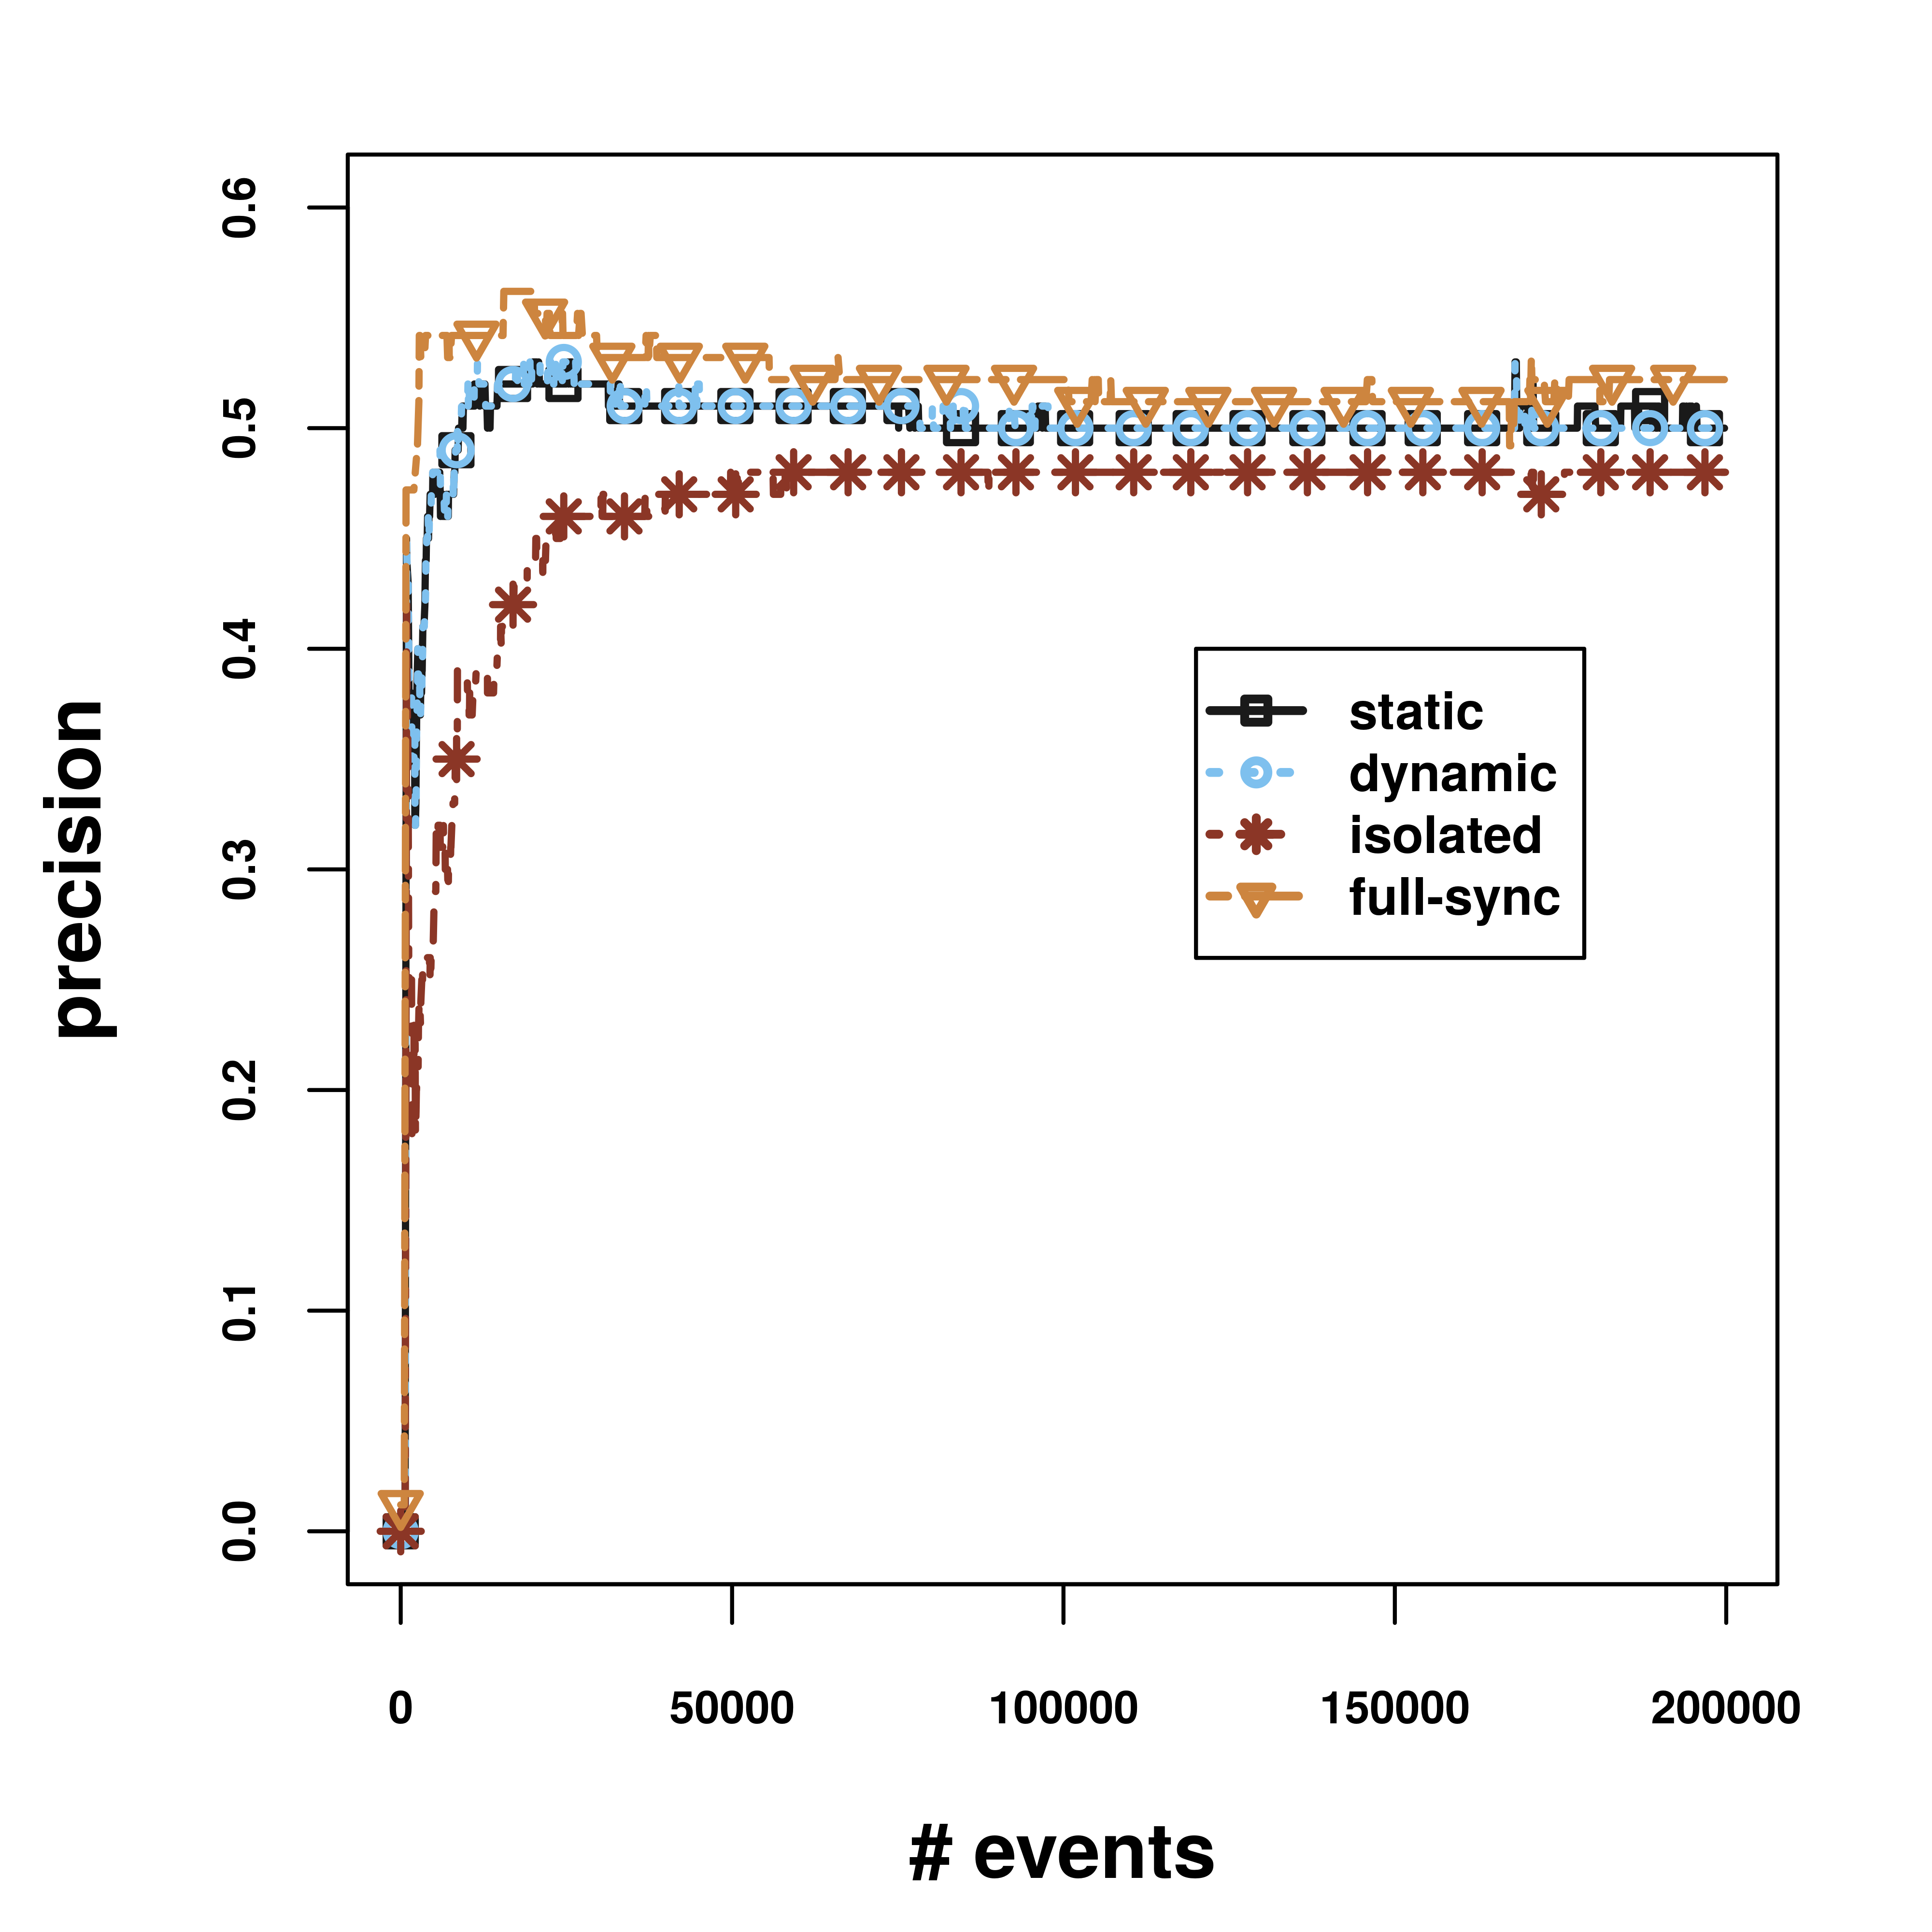
\includegraphics[width=.7\textwidth,height=.6\textheight]{../chapters/figures/synthetic/new/precision_synthetic.png}\linebreak\\
		Methods of distributed learning converge faster than the isolated method.
		
	\end{figure}
	
\end{frame}


\begin{frame}
	
	\frametitle{Results on Synthetic Event Streams }
	\framesubtitle{Average spread  with respect to the number of input events over time for $\mathcal{P}=a;d;c$.}
	
\begin{figure}[]
	\centering
	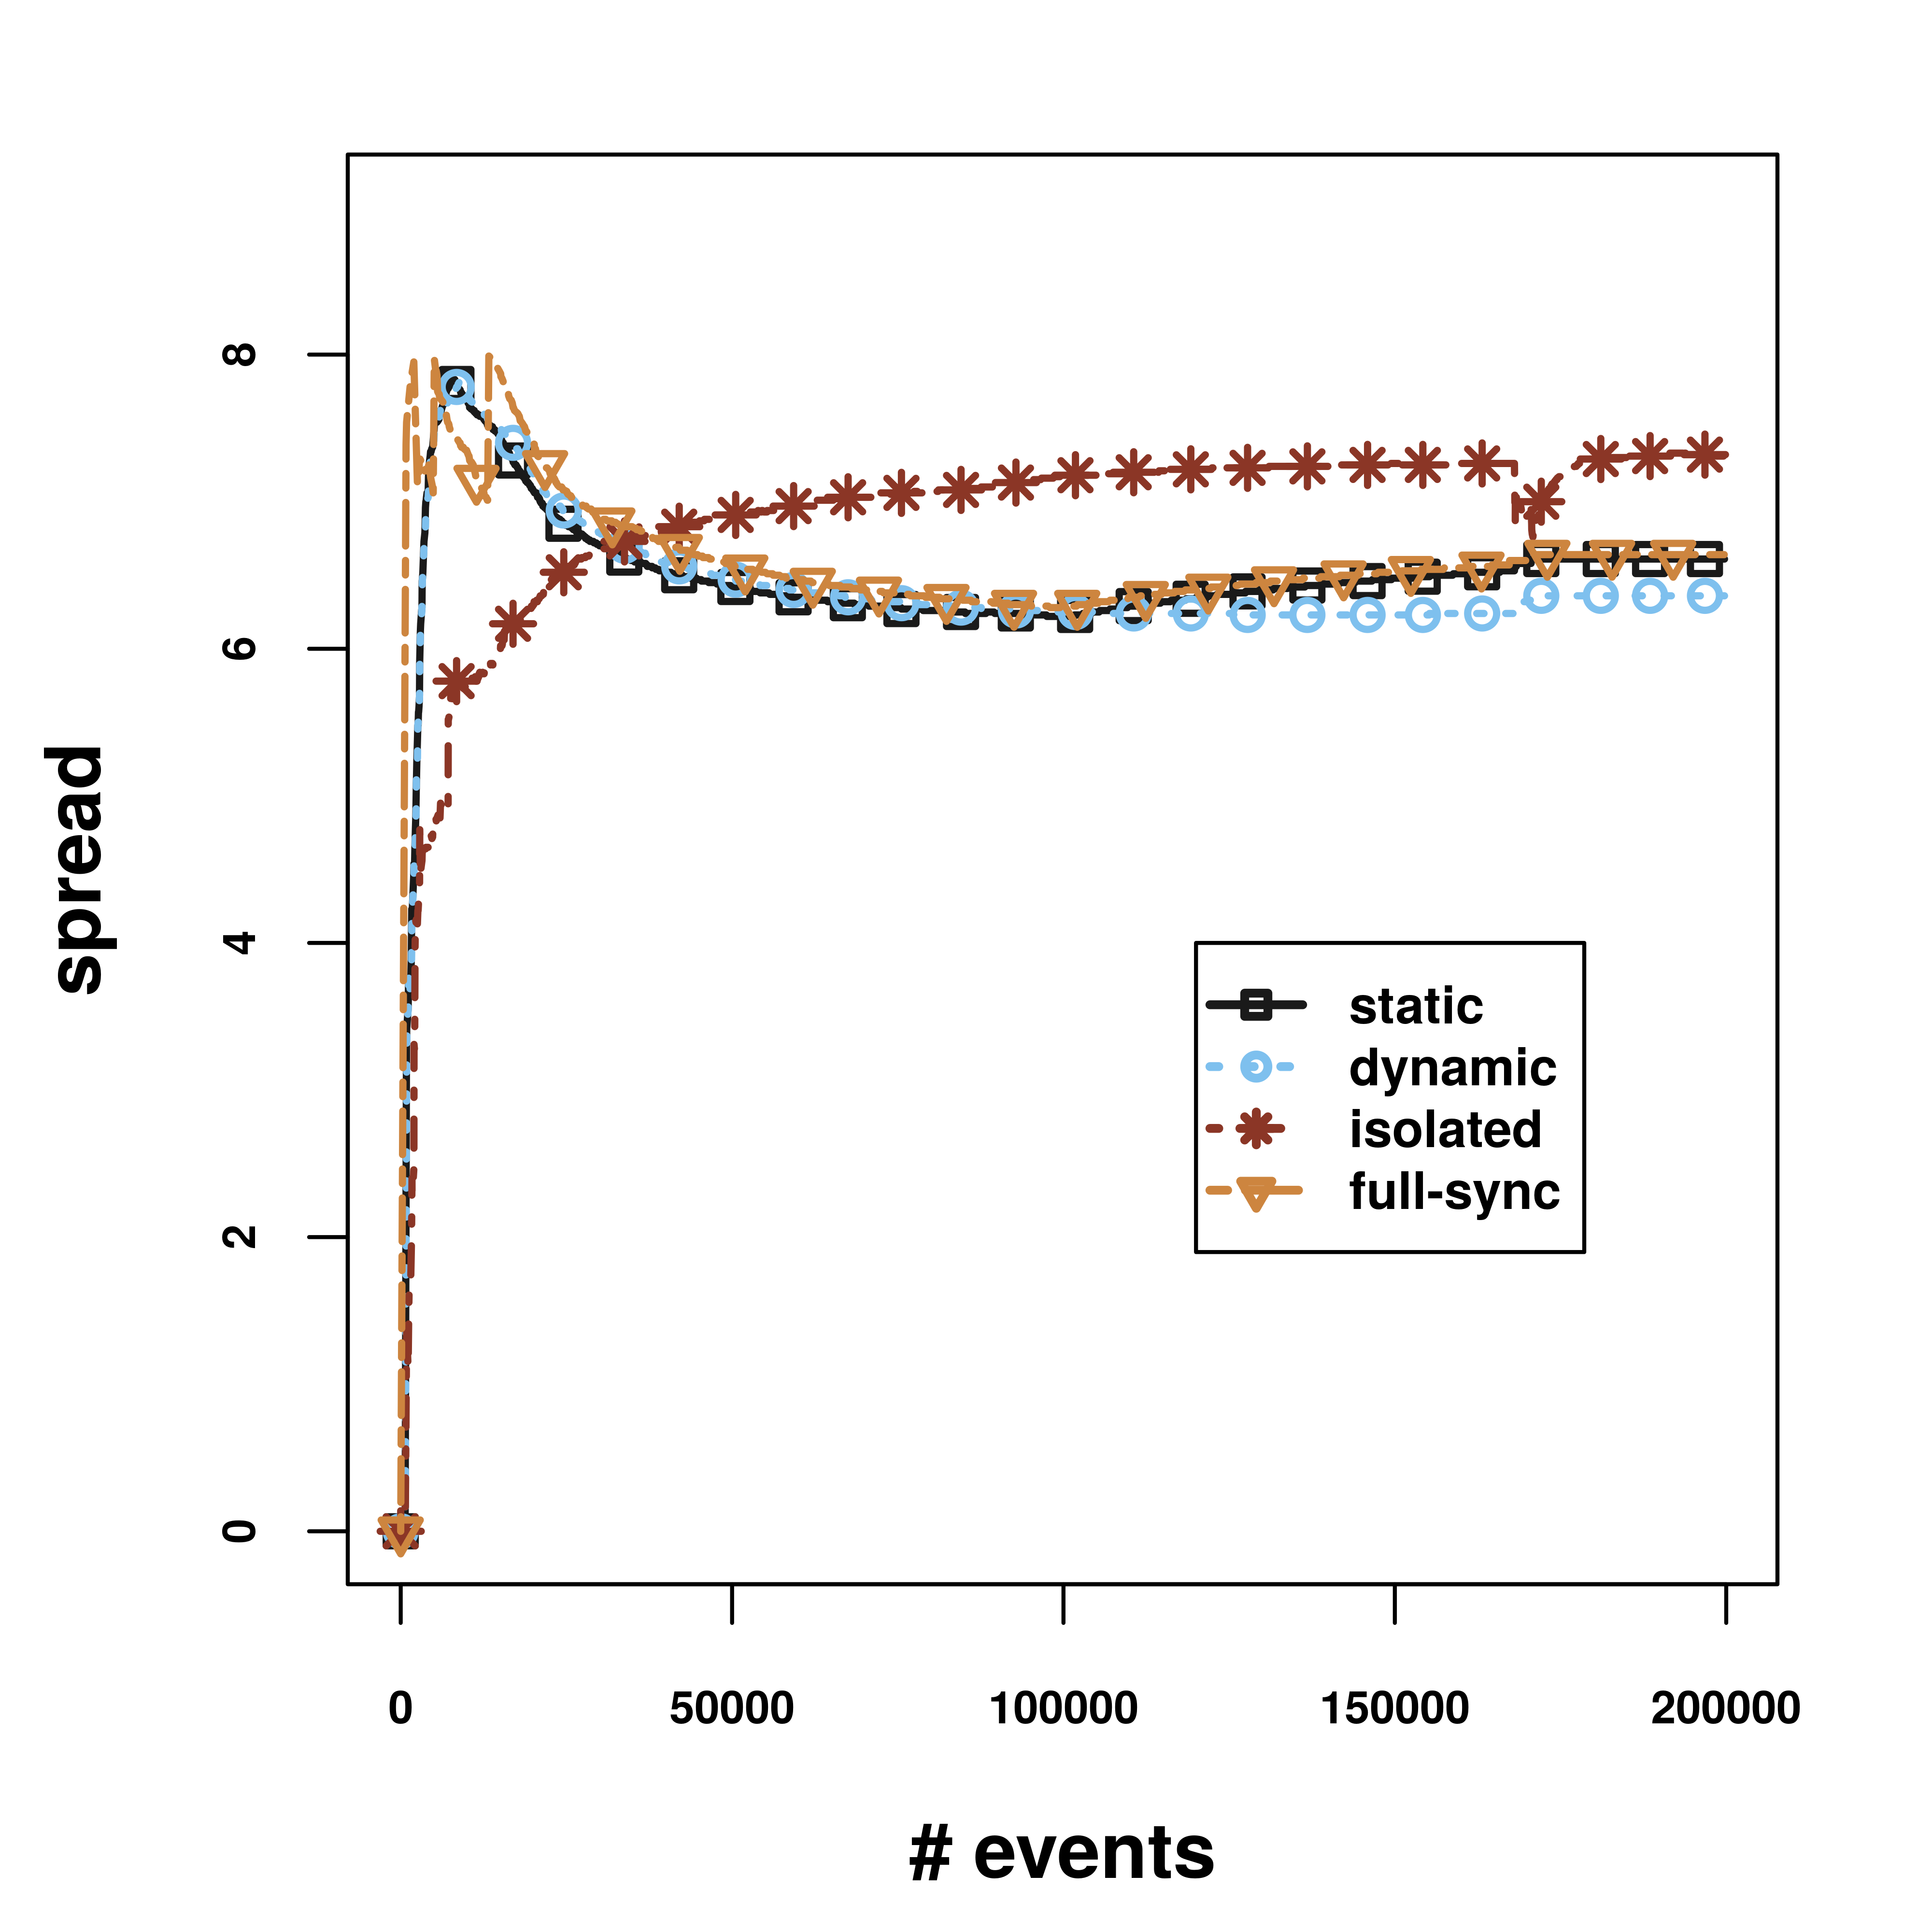
\includegraphics[width=.9\textwidth,height=.8\textheight]{../chapters/figures/synthetic/new/spread_synthetic.png}
	
\end{figure}
	
\end{frame}


\begin{frame}
	
	\frametitle{Results on Synthetic Event Streams }
	\framesubtitle{$\mathit{PS}$-score for $\mathcal{P}=a;d;c$ with $\alpha = .5$.}
	
\begin{figure}[H]
	\centering
	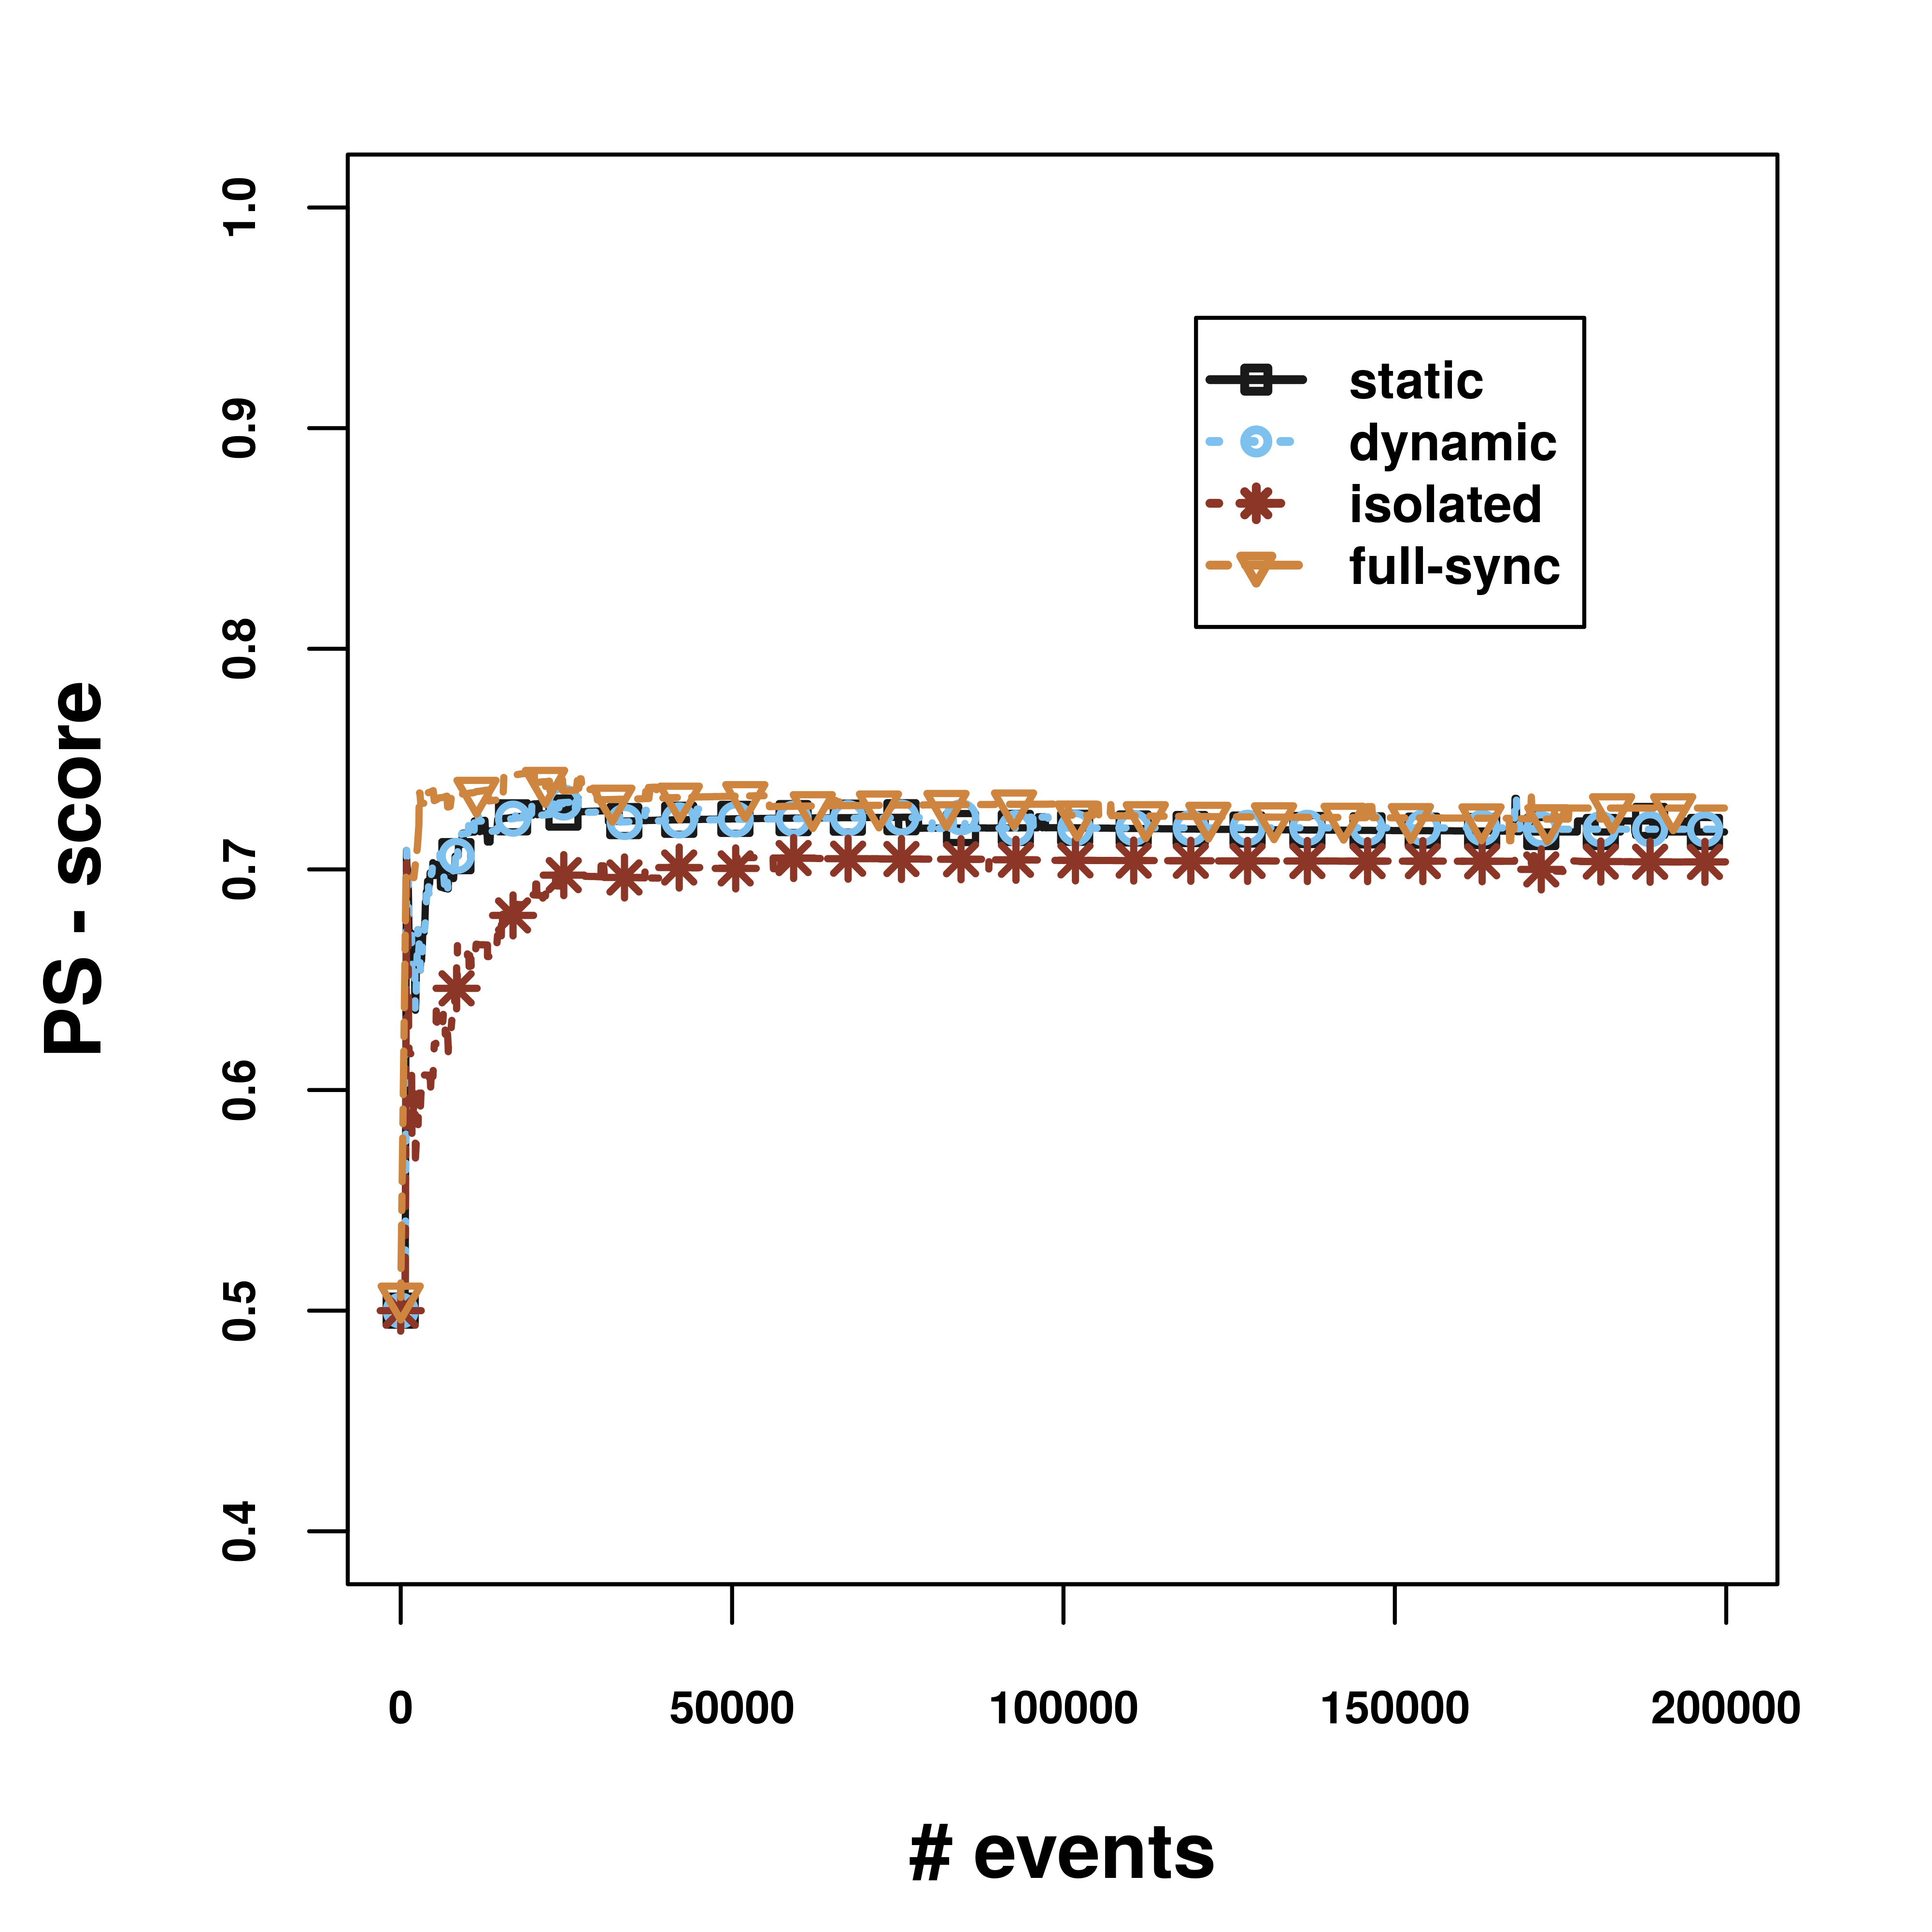
\includegraphics[width=.9\textwidth,height=.8\textheight]{../chapters/figures/synthetic/new/ps_score_synthetic.png}
	
\end{figure}
	
\end{frame}



\begin{frame}
	
	\frametitle{Results on Synthetic Event Streams }
	\framesubtitle{The error  $\sum_{i,j} |\hat{p}_{i,j} - {p}_{i,j}|$) of estimating the transition probabilities  for $\mathcal{P}=a;d;c$.}
	
	\begin{figure}[H]
		\centering
		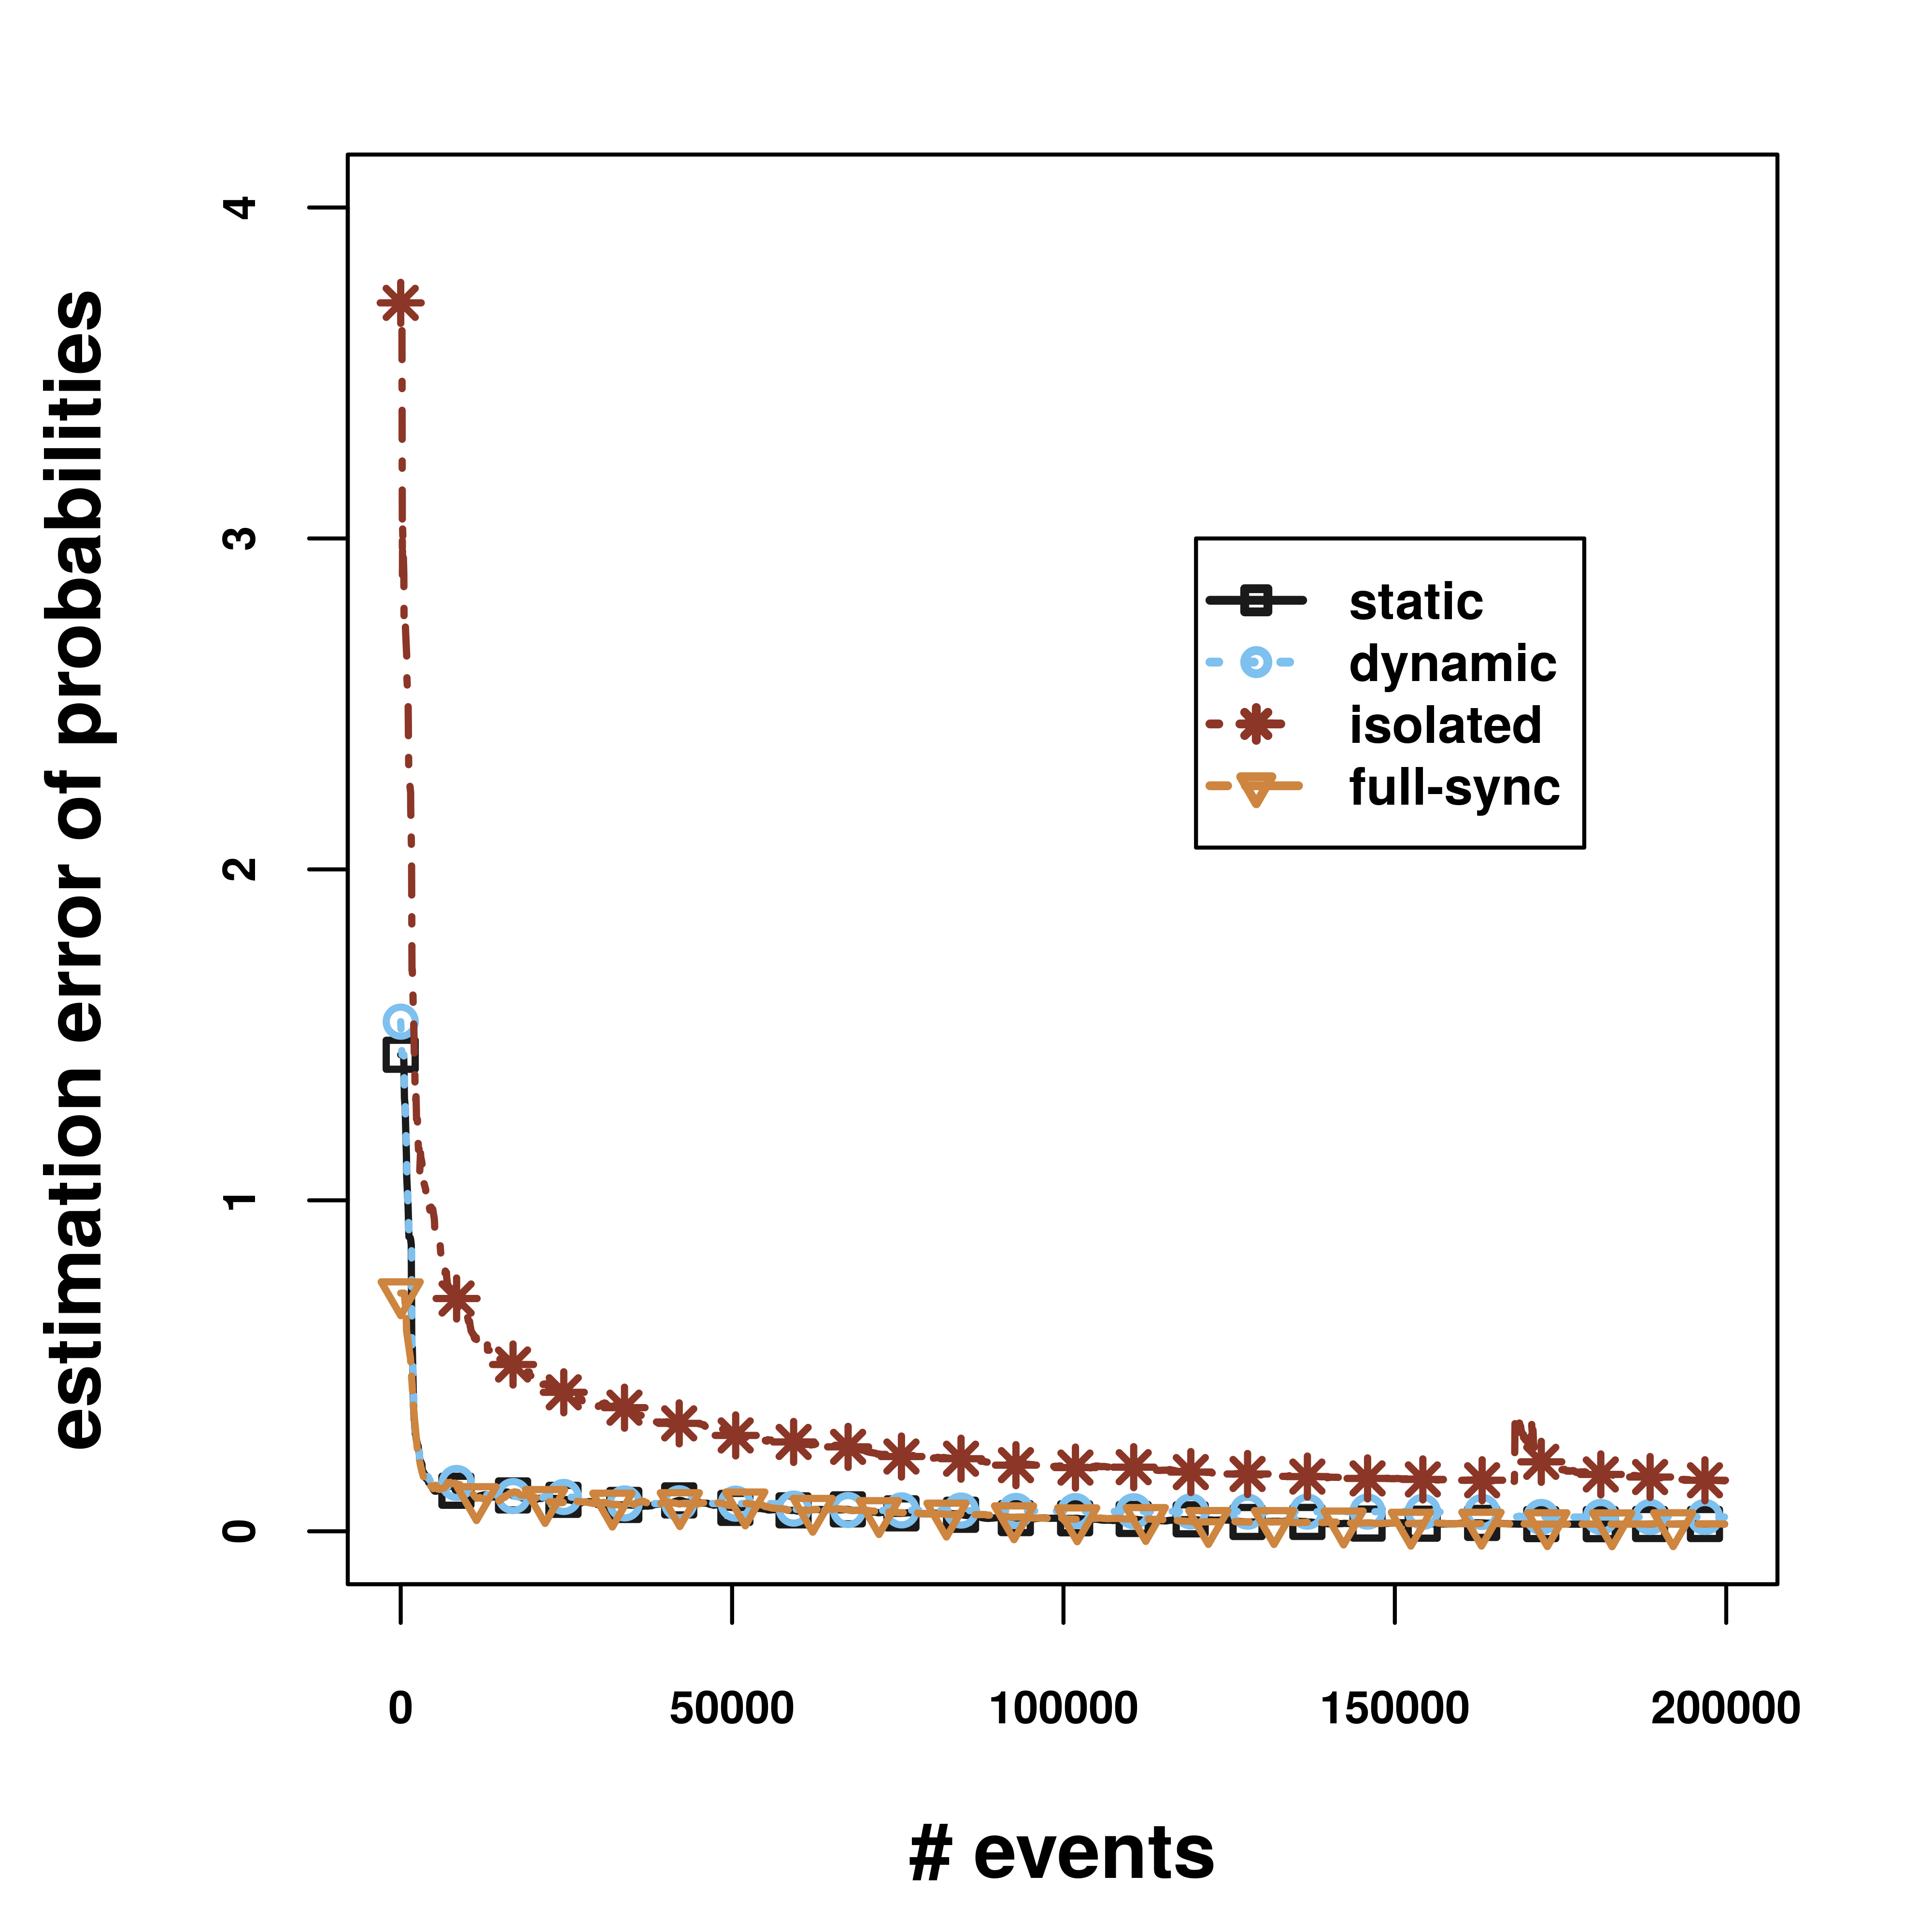
\includegraphics[width=.9\textwidth,height=.8\textheight]{../chapters/figures/synthetic/new/error_synthetic.png}
		
	\end{figure}
	
\end{frame}


\begin{frame}
	
	\frametitle{Throughput Results}
	\framesubtitle{Throughput of the system on YARN cluster in in terms of number of events processed per second with respect to the parallelism level over $\mathcal{P}_1$ with batch size $b=100$ and divergence threshold $\Delta=2$.}
	
	\begin{figure}[H]
		
		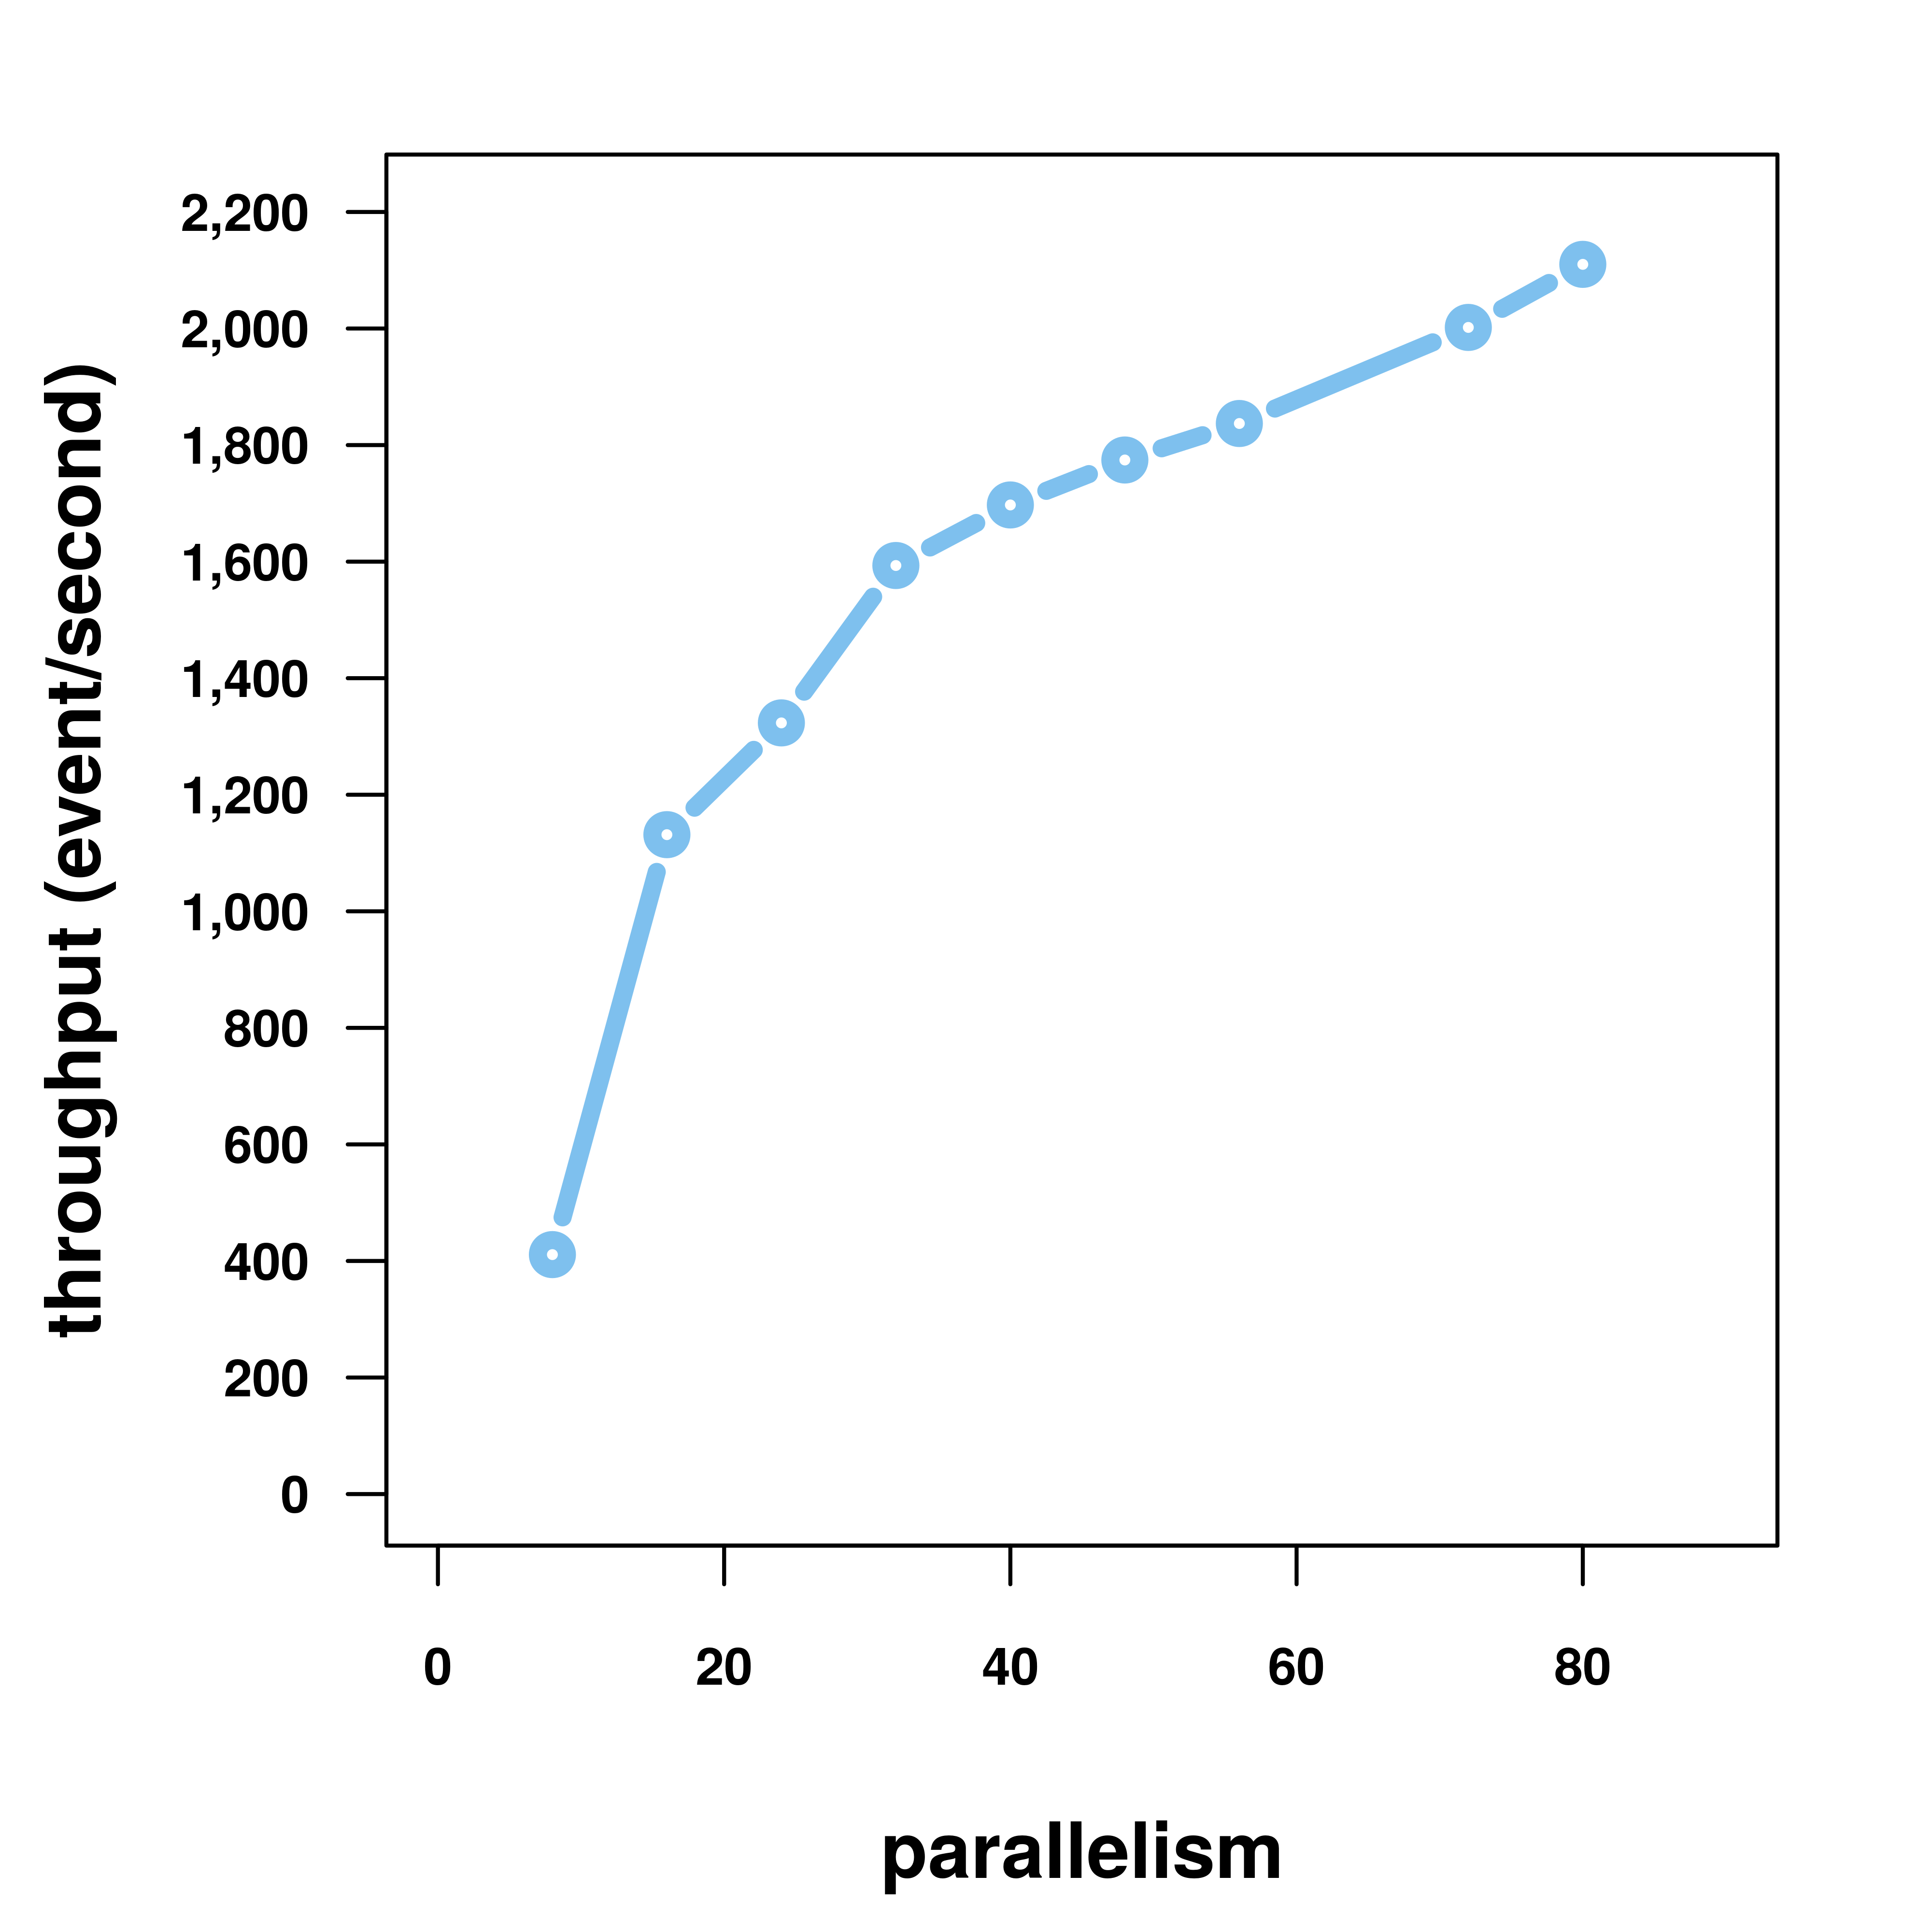
\includegraphics[width=.8\textwidth,height=.75\textheight]{../chapters/figures/throughput/temp.png}
		
	
	\end{figure}
	
\end{frame}